% Paquets généraux
\documentclass[a4paper,12pt,titlepage,twoside]{article}
\usepackage[T1]{fontenc}
\usepackage[utf8]{inputenc}
\usepackage[french]{babel}
\usepackage{subcaption}
\addto\captionsfrench{%
  \renewcommand{\tablename}{Tableau}%
}
\usepackage[gen]{eurosym}
%\usepackage[dvips]{graphicx}
\usepackage{minted}
\usepackage{fancyhdr}
\usepackage{pdfpages} 
\usepackage{multido}
\usepackage{hyperref}
\usepackage{textcomp}
\usepackage{schemabloc}
%\usepackage[bitstream-charter]{mathdesign}
\usepackage{array}
\newcolumntype{P}[1]{>{\centering\arraybackslash}p{#1}}
\usepackage[shortlabels]{enumitem}
\usepackage[framemethod=TikZ]{mdframed}

\newcommand{\id}{71}
\newcommand{\nom}{Théorie des mécanismes}
\newcommand{\sequence}{04}
\newcommand{\nomsequence}{Liaisons entre les solides}
\newcommand{\num}{02}
\newcommand{\type}{KH}
\newcommand{\descrip}{Liaisons équivalentes, hyperstatisme, liaisons en série et en parallèle, théorie des graphes}
\newcommand{\competences}{B2-12: Proposer une modélisation des liaisons avec leurs caractéristiques géométriques. \\ &  B2-13: Proposer un modèle cinématique paramétré à partir d'un système réel, d'une maquette numérique ou d'u \\ &  B2-17: Simplifier un modèle de mécanisme. \\ &  B2-18: Modifier un modèle pour le rendre isostatique. \\ &  C1-04: Proposer une démarche permettant d'obtenir une loi entrée-sortie géométrique.  \\ &  C2-05: Caractériser le mouvement d'un repère par rapport à un autre repère. \\ &  C2-06: Déterminer les relations entre les grandeurs géométriques ou cinématiques. }
\newcommand{\nbcomp}{7}
\newcommand{\systemes}{}
\newcommand{\systemesnum}{}
\newcommand{\systemessansaccent}{}
\newcommand{\ilot}{2}
\newcommand{\ilotstr}{02}
\newcommand{\dossierilot}{\detokenize{Ilot_02 }}

%\usepackage{style}
\usepackage{bodegraph}
\usepackage{rpcinematik}
\usepackage[locale = FR]{siunitx}
\usepackage{caption}
\newcommand{\institute}{Lycée Dorian}

\usepackage{listings}
\usepackage{fancyvrb}
\usepackage{color}
\usepackage{xcolor}
\usepackage{colortbl}
\usepackage{helvet}
\usepackage[frenchmath]{newtxsf} % for sans serif symbols
\renewcommand{\familydefault}{\sfdefault}
%\usepackage{amsfonts}
%\usepackage{amsmath}
%\usepackage{lmodern}
\usepackage{mathastext}
%\usepackage{xspace}
\usepackage{varioref}
\usepackage{tabularx}
%\usepackage{floatflt}
\usepackage{graphics}
\usepackage{wrapfig}
\usepackage{textcomp}
\usepackage{tikz,tkz-tab}
\usepackage[european resistor, european voltage, european current]{circuitikz}
\usepackage{wrapfig}
\usepackage{gensymb}
\usepackage[percent]{overpic}
\usetikzlibrary{babel}
\usepackage{ifthen}
\usepackage{cancel}
\usepackage{etoolbox}
\usepackage{multirow}
%\usepackage{boxedminipage}
\definecolor{gris25}{gray}{0.75}
\definecolor{bleu}{RGB}{18,33,98}
\definecolor{bleuf}{RGB}{42,94,171}
\definecolor{bleuc}{RGB}{231,239,247}
\definecolor{bleum}{RGB}{160,195,226}
\definecolor{rougef}{RGB}{185,18,27}
\definecolor{rougec}{RGB}{255,188,204}%255,230,231
\definecolor{vertf}{RGB}{103,126,82}
\definecolor{vertc}{RGB}{220,255,191}
\definecolor{forestgreen}{rgb}{0.13,0.54,0.13}
\definecolor{blcr}{rgb}{0.59,0.69,0.84}
\definecolor{blfr}{rgb}{0.32,0.51,0.75}
\definecolor{orfr}{rgb}{0.90,0.42,0.15}
\definecolor{orcr}{rgb}{0.90,0.65,0.50}
\definecolor{orangef}{rgb}{0.659,0.269,0.072}
\definecolor{orange}{rgb}{0.58,0.35,0.063}
\definecolor{orangec}{rgb}{0.43,0.32,0.25}
\definecolor{rcorrect}{rgb}{0.6,0,0}
\definecolor{sequence}{rgb}{0.75,0.75,0.75}
\definecolor{competences}{rgb}{0.61,0.73,0.35}
\definecolor{rose}{HTML}{ff00ff}
\definecolor{grisf}{HTML}{222222}
\definecolor{grisc}{HTML}{636363}
\definecolor{normal}{HTML}{4087c4}
\definecolor{info}{HTML}{5bc0de}
\definecolor{success}{RGB}{92,184,92}
\definecolor{warning}{RGB}{240,173,78}
\definecolor{danger}{RGB}{217,83,79}
\hypersetup{                    % parametrage des hyperliens
    colorlinks=true,                % colorise les liens
    breaklinks=true,                % permet les retours à la ligne pour les liens trop longs
    urlcolor= blfr,                 % couleur des hyperliens
    linkcolor= orange,                % couleur des liens internes aux documents (index, figures, tableaux, equations,...)
    citecolor= forestgreen                % couleur des liens vers les references bibliographiques
    }

\newcolumntype{M}[1]{>{\centering\arraybackslash}m{#1}}
\definecolor{codegreen}{rgb}{0,0.6,0}
\definecolor{codegray}{rgb}{0.5,0.5,0.5}
\definecolor{codepurple}{rgb}{0.58,0,0.82}
\definecolor{backcolour}{rgb}{0.95,0.95,0.92}

\lstdefinestyle{mystyle}{
    backgroundcolor=\color{backcolour},   
    commentstyle=\color{codegreen},
    keywordstyle=\color{magenta},
    numberstyle=\tiny\color{codegray},
    stringstyle=\color{codepurple},
    basicstyle=\ttfamily\footnotesize,
    breakatwhitespace=false,         
    breaklines=true,                 
    captionpos=b,                    
    keepspaces=true,                 
    numbers=left,                    
    numbersep=5pt,                  
    showspaces=false,                
    showstringspaces=false,
    showtabs=false,                  
    tabsize=2
}

\lstset{style=mystyle}

% Mise en page
\pagestyle{fancy}

\setlength{\hoffset}{-18pt}
\setlength{\oddsidemargin}{0pt} 	% Marge gauche sur pages impaire2s
\setlength{\evensidemargin}{0pt} 	% Marge gauche sur pages paires
\setlength{\marginparwidth}{00pt} 	% Largeur de note dans la marge
\setlength{\headwidth}{481pt} 	 	% Largeur de la zone de tête (17cm)
\setlength{\textwidth}{481pt} 	 	% Largeu\textbf{r de la zone de texte (17cm)
\setlength{\voffset}{-18pt} 		% Bon pour DOS
\setlength{\marginparsep}{7pt}	 	% Séparation de la marge
\setlength{\topmargin}{-30pt} 		% Pas de marge en haut
\setlength{\headheight}{55pt} 		% Haut de page
\setlength{\headsep}{20pt} 		% Entre le haut de page et le texte
\setlength{\footskip}{30pt} 		% Bas de\textbf{ page + séparation
\setlength{\textheight}{700pt} 		% Hauteur de l'icone zone de texte (25cm)
\setlength\fboxrule{1 pt}
\renewcommand{\baselinestretch}{1}
\setcounter{tocdepth}{1}
\newcommand{\cadre}[2]
{\fbox{
  \begin{minipage}{#1\linewidth}
   \begin{center}
    #2\\
   \end{center}
  \end{minipage}
 }
}

\newcommand{\repon}[1]
{
~\ \\
\begin{tabular}{|m{\linewidth}|}
 \hline
\multido{}{#1}{\\ \hline}
\end{tabular}
}


\newcommand{\objectif}[1]{
\mdfsetup{%
frametitle={%
\tikz[baseline=(current bounding box.east),outer sep=0pt]
\node[anchor=east,rectangle,fill=bleum]
{\strut Objectif~};}}
\mdfsetup{innertopmargin=10pt,linecolor=bleum,%
linewidth=2pt,topline=true,%
frametitleaboveskip=\dimexpr-\ht\strutbox\relax
}
\begin{mdframed}[]\relax%
#1
\end{mdframed}}


\newcounter{num_quest} \setcounter{num_quest}{0}
\newcounter{num_rep} \setcounter{num_rep}{0}
\newcounter{num_cor} \setcounter{num_cor}{0}

\newcommand{\feuilleDR}[1]{
	\begin{tikzpicture}
		\draw[gray!30](0,0)grid[step=0.5cm](\linewidth,#1);
	\end{tikzpicture}
}

%\newcommand{\question}[1]{\refstepcounter{num_quest}\par
%~\ \\ \parbox[t][][t]{0.15\linewidth}{\textbf{Question \arabic{num_quest}}}\parbox[t][][t]{0.85\linewidth}{#1\label{q\the\value{num_quest}}}\par
%}

\newcommand{\question}[1]{\refstepcounter{num_quest}\par
~\ \\ \textbf{Question \arabic{num_quest} : }#1\label{q\the\value{num_quest}}\par
}

\newcommand{\posetafigure}[3]{
\begin{figure}[ht!]
 \begin{center}
  \includegraphics[width=#2\linewidth]{img/#1}
 \end{center}
 \caption{\label{#1} #3}
\end{figure}}

\newcommand{\goforum}{
\begin{figure}

\end{figure}
\begin{center}
 
\includegraphics[width=0.7\linewidth]{../../../img/go_forum}
\end{center}
\label{go_forum}
\caption{J'pète les plombs}
\end{figure}}

\newcommand{\reponse}[4][1]
{\noindent
\parbox{\textwidth}{
\rule{\linewidth}{.5pt}\\
\textbf{Question\ifthenelse{#1>1}{s}{} \multido{}{#1}{%
\refstepcounter{num_rep}\ref{q\the\value{num_rep}} }:} ~\ \\
\ifdef{\public}{#3 \ifthenelse{#2>0}{~\ \\ 	\feuilleDR{#2}}}{#4}
}}

\newcommand{\cor}
{\refstepcounter{num_cor}
\noindent
\rule{\linewidth}{.5pt}
\textbf{Question \arabic{num_cor}:} \\
}

\newcommand{\finsujet}
{
    \begin{center}
    \Large{FIN}
    \end{center}

    \cleardoublepage

    \ifdef{\public}{\pagestyle{docreponse}}{\pagestyle{correction}}

    \ifdef{\public}{
        \begin{tikzpicture} 
            \draw (0,0) rectangle (2,2);
            \draw (0,0) -- (2,2);
            \draw (1.5,0.5) node {\large 20};
            \draw (2.5,0) rectangle (16,2);
            \draw (4.5,1.7) node {\large Commentaires:};
        \end{tikzpicture}
    }
    ~\ \\
}


%\newcommand{\repcarre}[2]
%{
%~\ \\
%\begin{tikzpicture}
%\draw [fill=white] (0,0) rectangle +(\linewidth,#1);
%\node[align=left] at (1.1,#2-0.3) {\textbf{Question #1:}};
%\end{tikzpicture}
%}

\newcommand{\titre}[1]
{\begin{center}
\cadre{0.8}{\huge #1} 
\end{center}
}


%Définition des torseurs :
\newcommand{\torseur}[2]{\left\{\mathcal{#1}_{#2} \right\}}
\newcommand{\torseurh}[3]{\left\{\genfrac{}{}{0pt}{0}{#1}{#2}\right\}_{#3}}
\newcommand{\torseurv}[8]{\left\{
\begin{matrix}
#1 & #4 \\ #2 & #5 \\ #3 &#6
\end{matrix}
\right\}_{{#7},{#8}}}

%Définition des torseurs :
%\newcommand{\torseur}[2]{\left \{\mbox{\relsize{2}{$\mathcal {#1}$}\relsize{-2}}\phantom{}_{\mbox{\scriptsize $#2$}} \right \}}
%\newcommand{\torseurh}[3]{\left\{\genfrac{}{}{0pt}{0}{#1}{#2}\right\}_{#3}}
%\newcommand{\torseurv}[8]{
%\left\{\begin{array}{@{}c|c@{}} #1 & #4 \\ #2 & #5 \\ #3 & #6 \end{array} \right\}_{#7,#8}
%}
\newcommand{\derivee}[2]{\left.\dfrac{\d #1}{\d t}\right|_{#2}}
\newcommand{\tripleint}{\int\!\!\!\!\!\int\!\!\!\!\!\int}

% Notation cinématique et statique
\newcommand{\cinematique}[2]{\mbox{#1}/\mbox{#2}}
\newcommand{\statique}[2]{\mbox{#1}\rightarrow\mbox{#2}}
\newcommand{\moment}[3]{\vv {#1}_{\scriptsize{#3}}(#2)}
\newcommand{\resultante}[2]{\vv {#1}_{\scriptsize{#2}}}


%Commande de base
\newcommand{\jo}{\left(j\omega\right)} % j \omega dans l'analyse fréquentielle
\newcommand{\tl}{\xrightarrow{\mathcal{L}}} % transformée de laplace sur fleche
\newcommand{\tli}{\xrightarrow{\mathcal{L}^{-1}}} % transformée inverse de laplace sur fleche
\renewcommand{\d}[1][]{\mathrm{d#1}}
\newcommand{\dd}[1][]{\mathrm{d#1}}
\newcommand{\vect}[2]{{#1}\wedge{#2}}
\newcommand{\base}[3]{(\vec #1,\vec #2,\vec #3)}
\newcommand{\vectbase}[4]{{\vphantom{\left| \begin{matrix}
#1\\#2\\#3 \end{matrix} \right|}}_{#4}{\left| \begin{matrix}
#1\\#2\\#3 \end{matrix} \right.}}
%Pour avoir les paragraphes sous la forme I, II, III
\renewcommand{\thesection}{\Roman{section}}
\setcounter{secnumdepth}{3}
\renewcommand{\Frlabelitemii}{$\bullet$}

% En tête et pied de page
\lhead{\nom}
\rhead{
\includegraphics[width=2cm]{../../../img/logo}}
\lfoot{\auteurun,\ \auteurdeux}
\cfoot{Page \thepage}

\fancypagestyle{docreponse}{%
  \fancyhf{}
  \fancyhead[LO]{NOM Prénom: .............................}
  \rhead{
\includegraphics[width=2cm]{../../../img/logo}\hspace{2pt}}
  \ifdef{\auteurdeux}{\lfoot{\auteurun,\ \auteurdeux}}{\lfoot{\auteurun}}
  \rfoot{\nom}
  \lfoot{Document réponse}
  \cfoot{Page \thepage}
   }

\fancypagestyle{correction}{%
  \fancyhf{}
  \lhead{\colorbox{danger}{\begin{minipage}{0.65\paperwidth} \textcolor{white}{\textbf{Correction}} \end{minipage}} }
  \rhead{
\includegraphics[width=2cm]{../../../img/logo}}
  \lfoot{Renaud Costadoat, Françoise Puig}
  \rfoot{\colorbox{danger}{\begin{minipage}{0.4\paperwidth} \begin{flushright}\textcolor{white}{\textbf{Correction}}\end{flushright} \end{minipage}} }}

\fancypagestyle{correctioninfo}{%
  \fancyhf{}
  \lhead{\colorbox{danger}{\begin{minipage}{0.65\paperwidth} \textcolor{white}{\textbf{Correction}} \end{minipage}} }
  \rhead{
\includegraphics[width=2cm]{../../../img/logo}}
  \lfoot{Renaud Costadoat, Juliette Genzmer}
  \rfoot{\colorbox{danger}{\begin{minipage}{0.6\paperwidth} \begin{flushright}\textcolor{white}{\textbf{Correction}}\end{flushright} \end{minipage}} }}

\renewcommand{\footrulewidth}{0.4pt}

\usepackage{eso-pic}
\newcommand{\BackgroundPic}{%
\put(0,0){%
\parbox[b][\paperheight]{\paperwidth}{%
\vfill
\begin{center}
\hspace{0.5cm}\vspace{0.5cm}

\includegraphics[width=\paperwidth,height=\paperheight,%
keepaspectratio]{../../../img/fond3}%
\end{center}
\vfill
}}}

\newcommand{\BackgroundPicdeux}{%
\put(25,-30){%
\parbox[b][\paperheight]{\paperwidth}{%
\vfill
\begin{center}
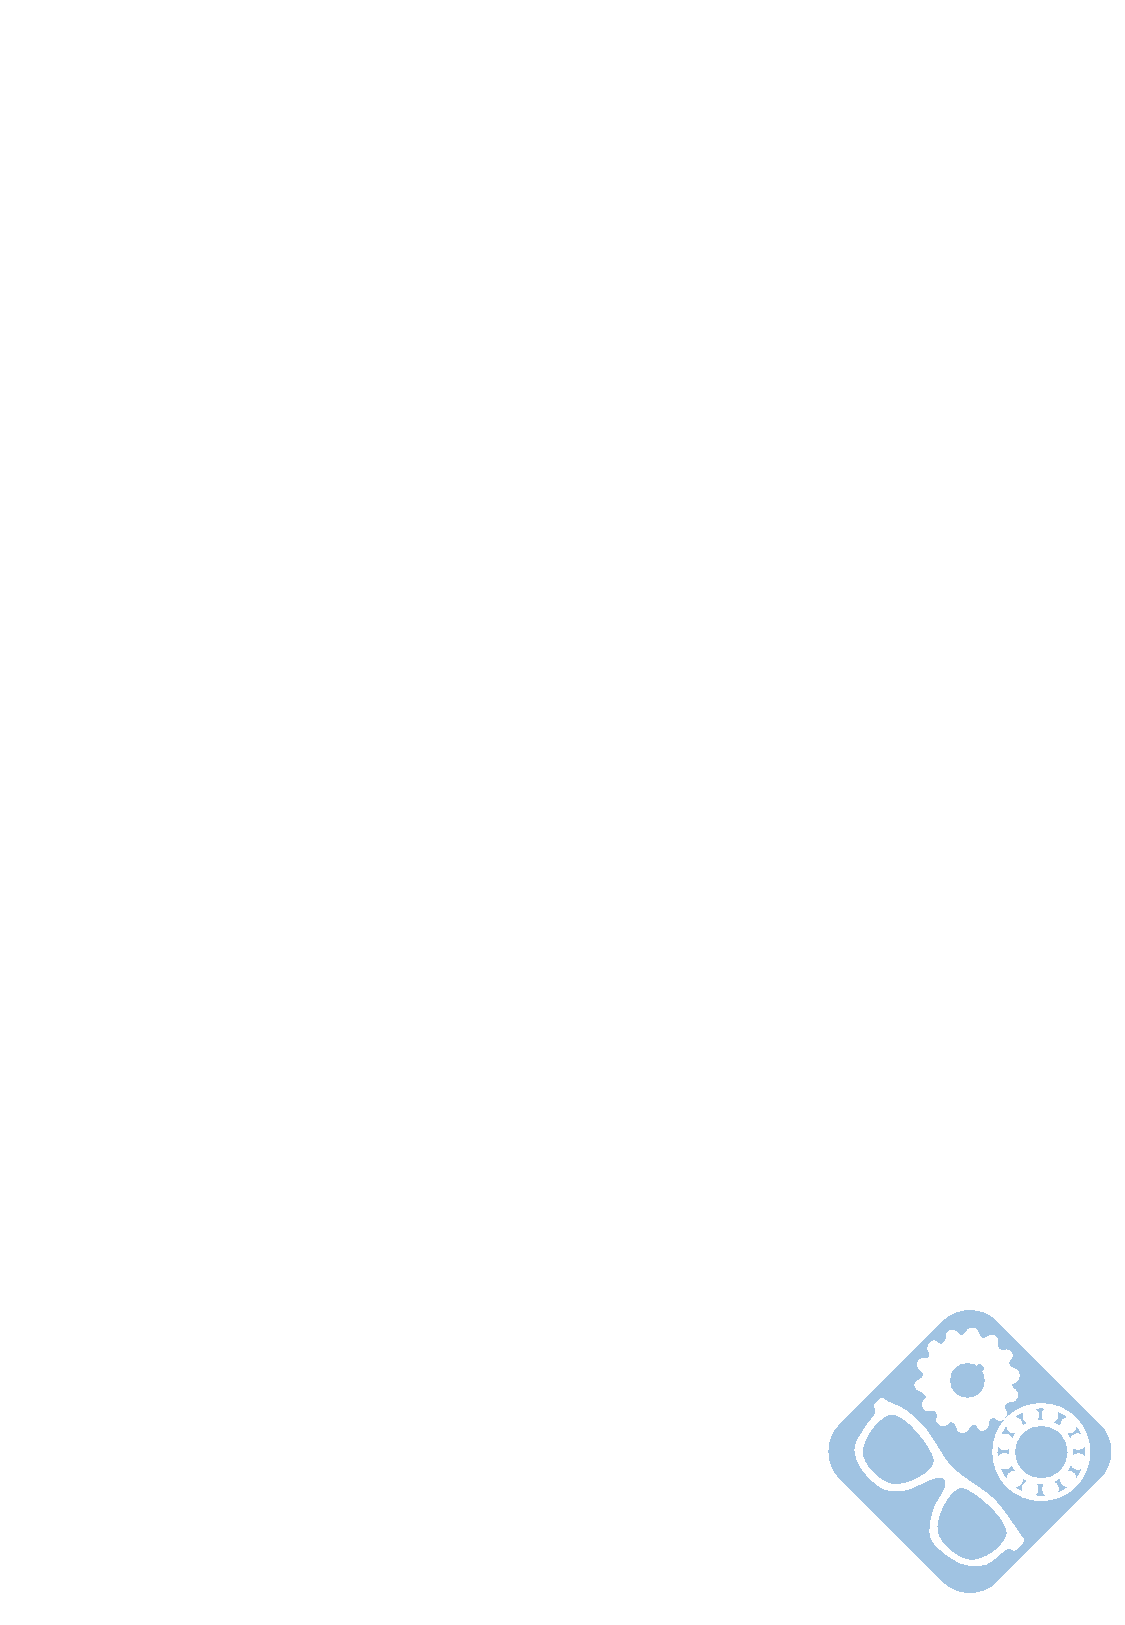
\includegraphics[width=\paperwidth,height=\paperheight,%
keepaspectratio]{../../../img/fond4}%
\end{center}
\vfill
}}}

\begin{document}

\pagestyle{empty}

\AddToShipoutPicture*{\BackgroundPic}


\includegraphics[width=2cm]{../../../img/logo}

\Huge{DS \numero - \sujet}

\vspace{1cm}

\ifdef{\prive}{\begin{center}\colorbox{danger}{\Huge{Avec Correction}}\end{center}}{}

\begin{center}
\centering\huge{PTSI}
\end{center}

\vspace{2cm}


\begin{center}
\centering\Large{\jour}
\end{center}

\vspace{2cm}

\normalsize

\tableofcontents

\newpage

\AddToShipoutPicture{\BackgroundPicdeux}

\pagestyle{fancy}

\begin{center}
\Huge \sujet
\end{center}


\normalsize


\section*{Contexte}

\begin{center}
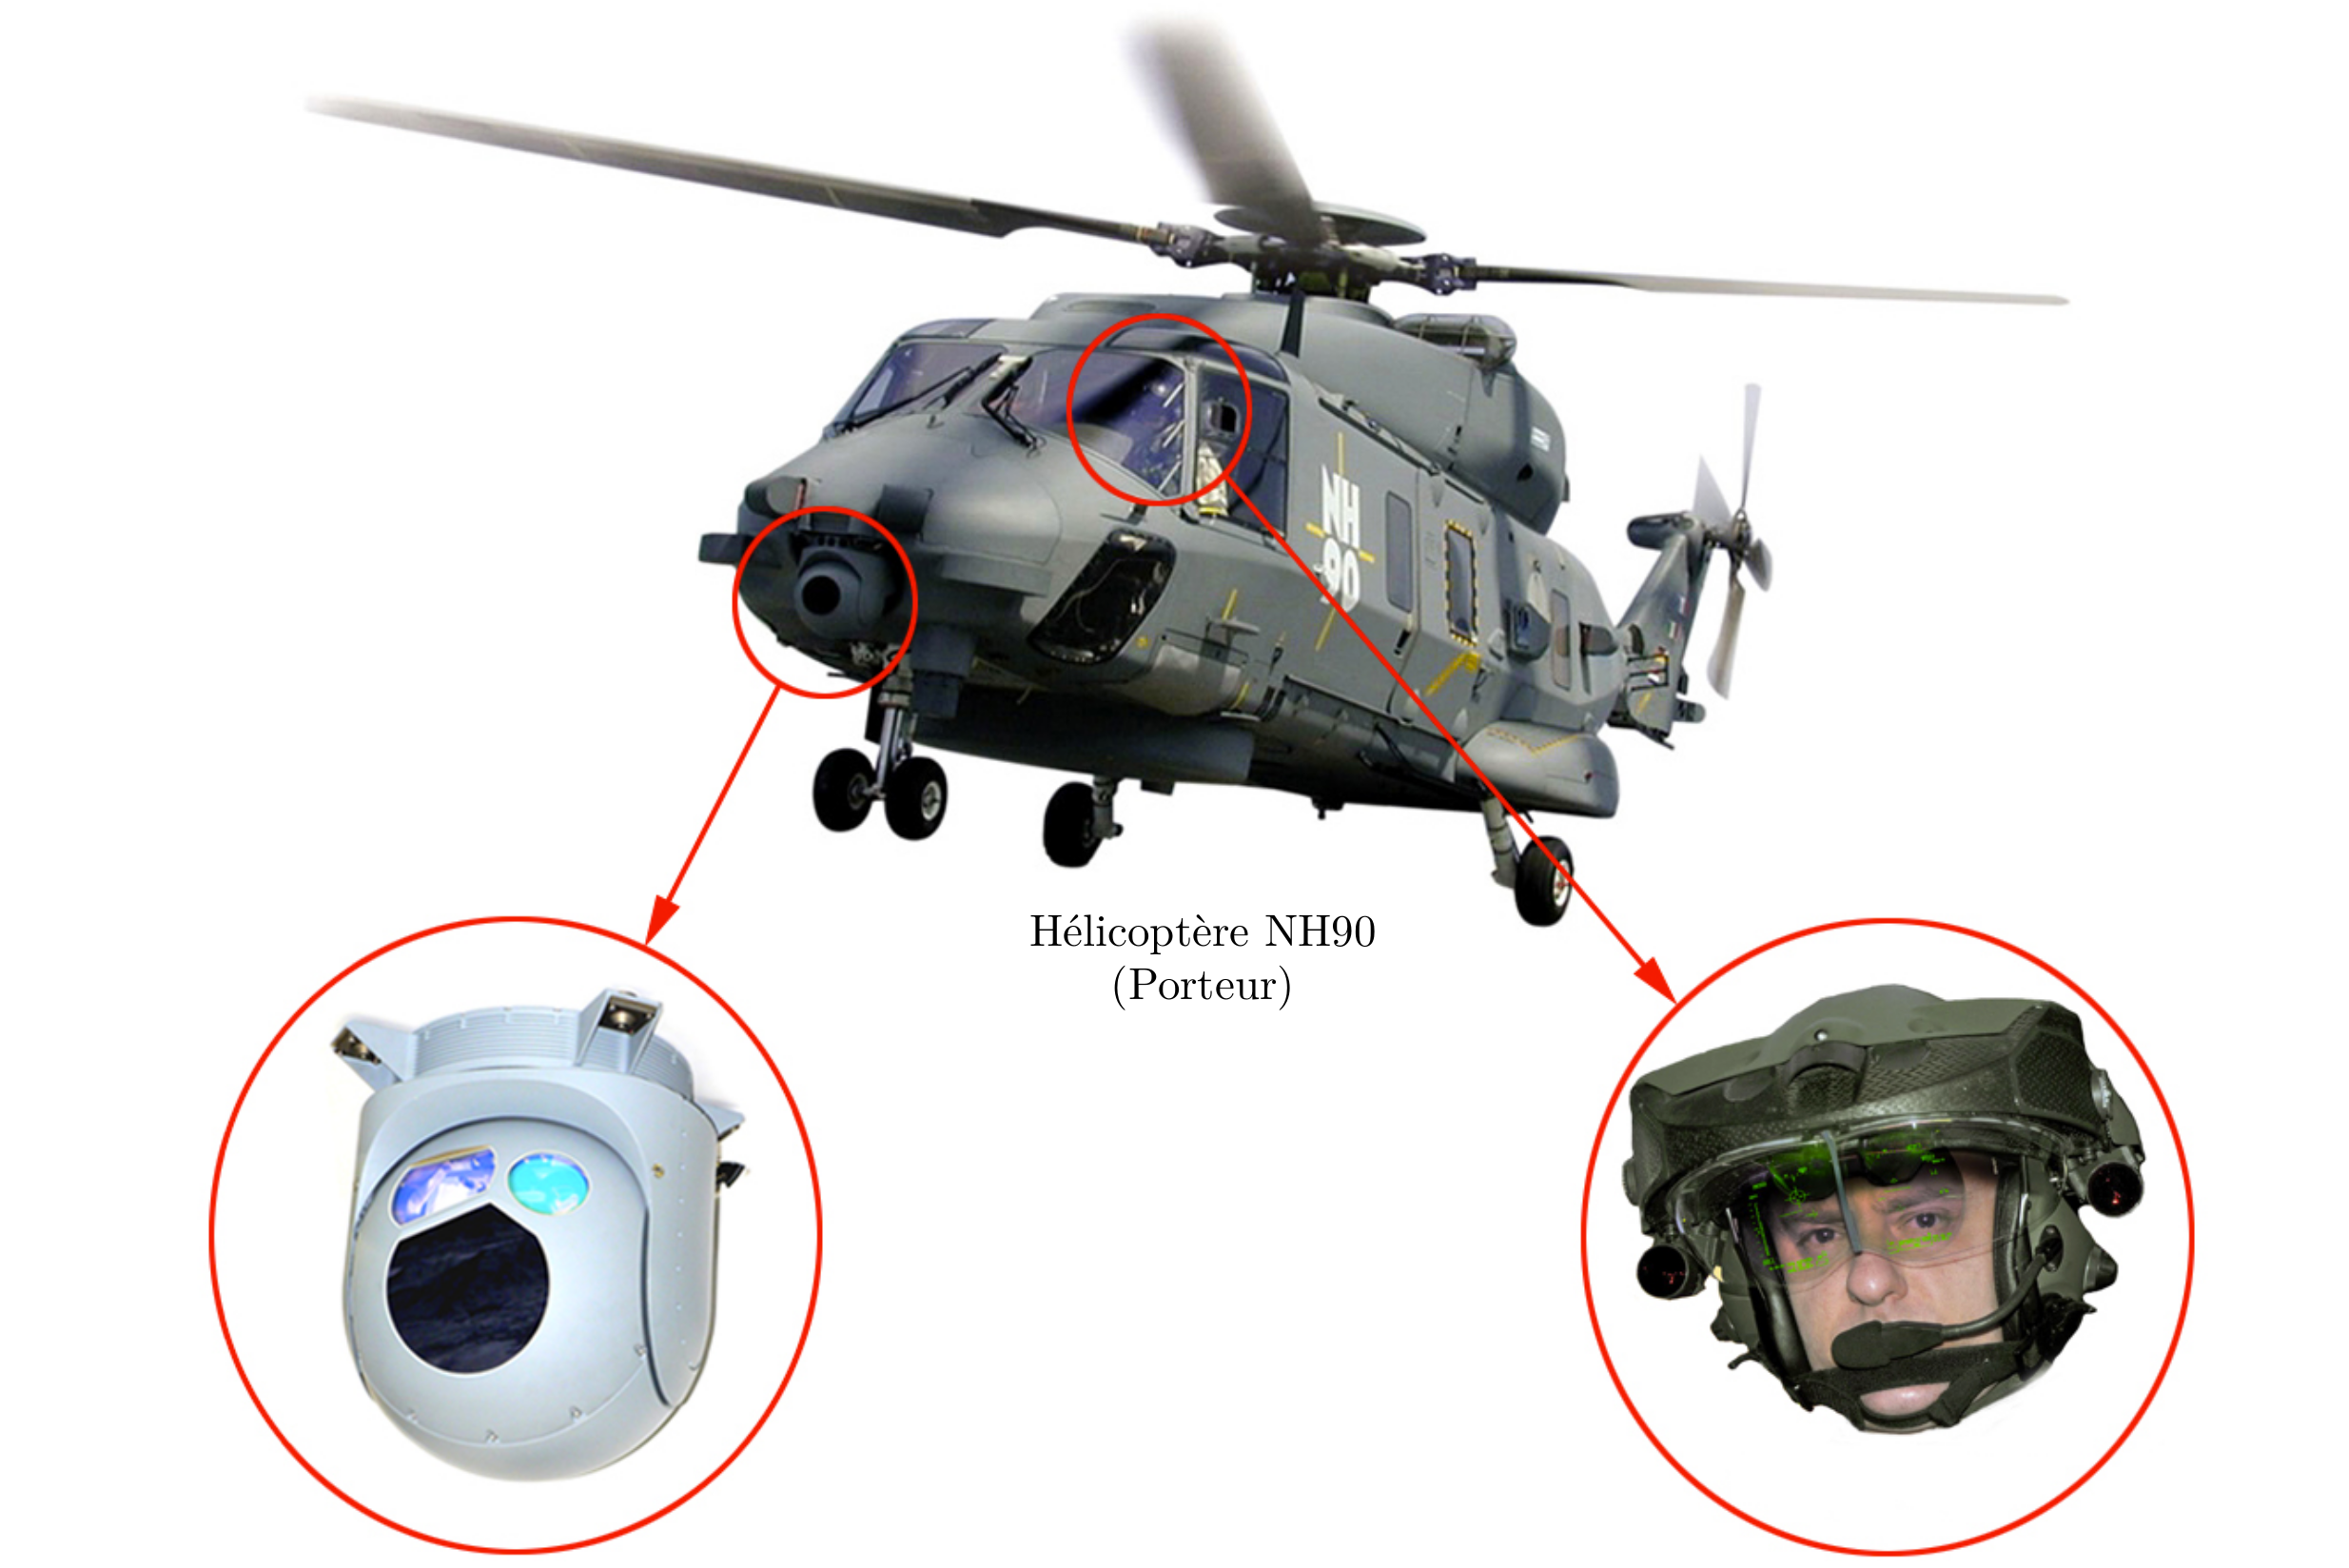
\includegraphics[width=0.7\linewidth]{img/fig01}
\captionof{figure}{\label{fig01}Hélicoptère NH90 équipé du système de vision en réalité augmentée}
\end{center}

Les hélicoptères sont des aéronefs dont l'un des intérêts est de pouvoir effectuer des vols proches du relief. Suivant les conditions climatiques (tempête de sable, brouillard ou vol de nuit par exemple), la propre vision du pilote et l'instrumentation de navigation classique peuvent être insuffisantes pour assurer la sécurité du vol. Pour pallier cela, la société Thalès propose un système de vision en réalité augmentée composée du casque TopOwl et d'un FLIR (Forward Looking InfraRed).

La vision en réalité augmentée consiste à venir projeter sur la visière du casque TopOwl une image prise par une des caméras du FLIR. L'image projetée se superpose au paysage visible à travers la visière de façon à améliorer la vision du pilote. De nuit, par temps de brouillard ou de tempête, l'image peut être une image infra-rouge ou thermique. En plus de l'image, des informations peuvent être ajoutées sur la projection ; par exemple des données GPS, des routes, des informations de vol.

\begin{center}
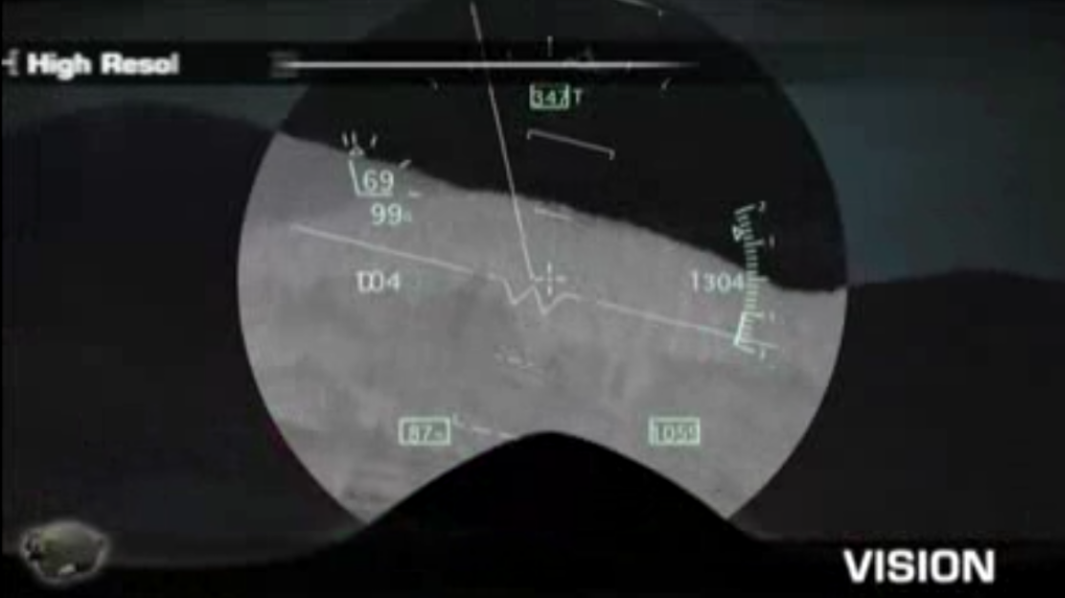
\includegraphics[width=0.5\linewidth]{img/fig02}
\captionof{figure}{\label{fig02}Vision nocturne et affichage des informations de vol}
\end{center}

Le FLIR est une boule optronique modulaire pouvant intégrer plusieurs capteurs différents dont une caméra thermique, une caméra couleur TV HD, ainsi qu'une caméra très bas niveau de lumière. Cet ensemble est orientable et gyrostabilisé, c'est-à-dire en particulier que les caméras sont capables de garder une même ligne de visée par rapport au référentiel terrestre, quels que soient les mouvements de l'hélicoptère NH90 qui sera appelé porteur dans la suite du sujet. Le casque TopOwl est placé sur la tête du pilote et le FLIR sur l'avant du porteur.

Une étude relative à la physique du casque TopOwl a permis de déterminer certaines de ses performances qui seront données au moment opportun. Ce sujet a pour objet l'étude des performances du sous-système FLIR, intégré dans le système de vision en réalité augmentée. La problématique globale est de vérifier que l'image projetée sur la visière du casque TopOwl est utilisable par le pilote, c'est-à-dire :
\begin{itemize}
 \item que la ligne de visée des caméras est conforme à la ligne de visée du pilote (les lignes de visée sont définies par rapport au référentiel terrestre) ;
 \item que le retard entre la prise de vue et son affichage n'est pas visible par le pilote (retard inférieur à la persistance rétinienne) ;
 \item que la prise de vue n'est pas perturbée par les mouvements du porteur.
\end{itemize}

\begin{center}
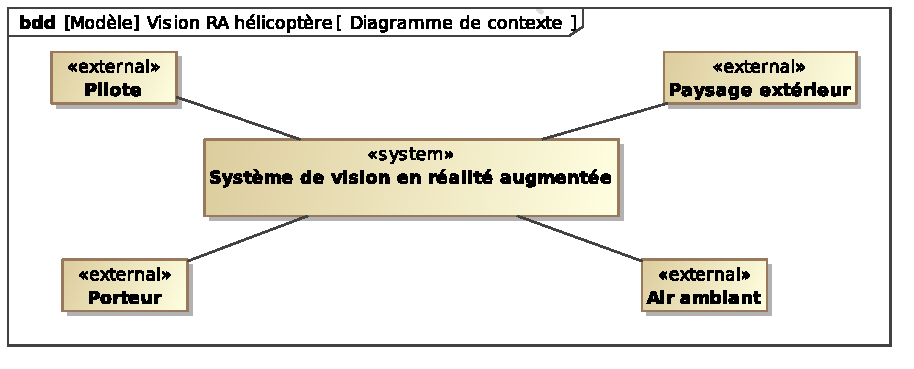
\includegraphics[width=0.7\linewidth]{img/Diagramme_de_contexte}
\captionof{figure}{\label{fig03}Diagramme de contexte du système}
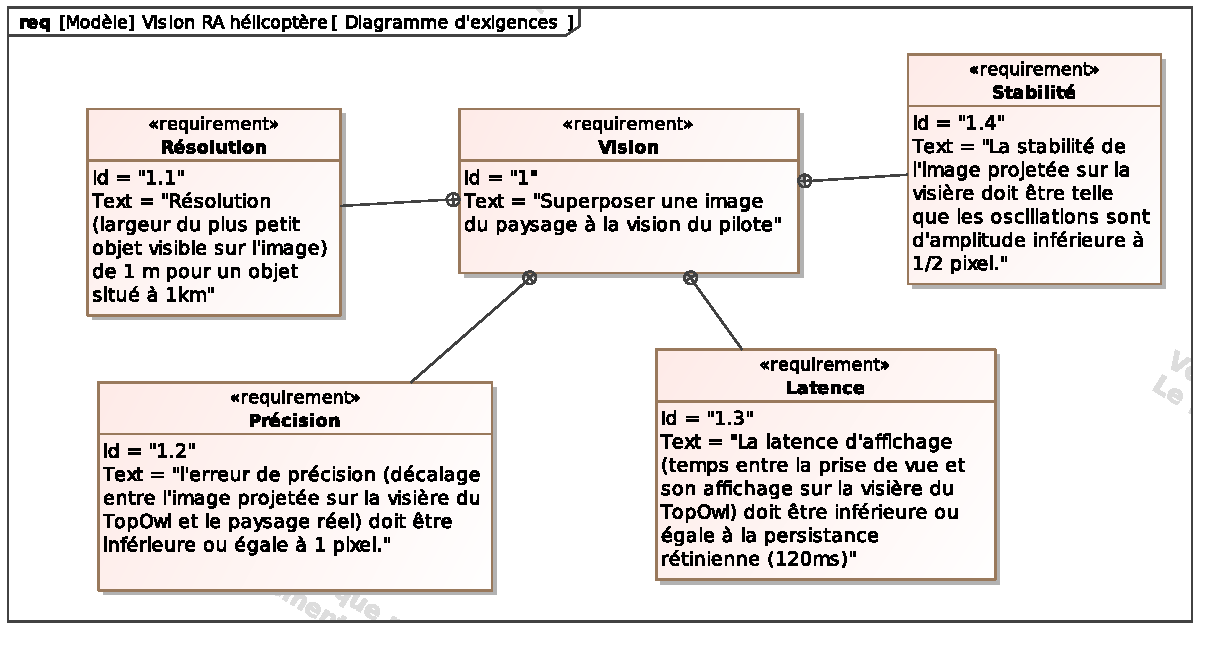
\includegraphics[width=0.7\linewidth]{img/Diagramme_d_exigences}
\captionof{figure}{\label{fig04}Diagramme d'exigences du système}
\end{center}

L'étude se décompose en trois parties. La partie I porte sur la détermination des performances (rapidité et précision) à atteindre par le sous-système FLIR en fonction du cahier des charges du système de vision en réalité augmentée et des performances des autres sous-systèmes. L'objectif de la partie II est d'analyser le choix d'architecture du FLIR en vue de valider les hypothèses simplificatrices concernant son comportement. La partie III consiste à vérifier si les solutions retenues, tant au niveau de l'architecture que de la commande, permettent d'atteindre
les performances attendues du FLIR.

\section{Performances attendues du sous-système FLIR intégré au système de vision en réalité augmentée}

\paragraph{Objectif}

Déterminer les performances de rapidité et de précision d'orientation de la ligne de visée du sous-système FLIR qui permettent de satisfaire le cahier des charges du système de vision en réalité augmentée pour hélicoptère.

\subsection{Validation des performances simulées du FLIR}


Le sous-système de détection de posture, appelé DDP, placé sur le casque TopOwl permet d'acquérir l'orientation spatiale de la tête du pilote par rapport au cockpit du porteur (3 angles de rotation). Cette information, couplée à l'information de position et d'orientation du porteur par rapport à la Terre (délivrée par une centrale inertielle fixée au porteur), permet d'élaborer la commande d'orientation du FLIR afin que sa ligne de visée corresponde à la ligne de visée du pilote. À partir d'un algorithme, une centrale de traitement d'image permet de calculer l'image à afficher sur la visière du casque TopOwl et les informations éventuelles à ajouter, comme celles issues de la position GPS par exemple.

\subsection{Détermination des performances du FLIR}

Une étude préalable a permis de déterminer que le système de détection de posture (DDP) a besoin d'un temps noté $t_{ddp}$ égal à 20 ms pour acquérir l'information. De même, le temps de traitement de l'information par filtrage noté $t_{filtre}$ est égal à 5 ms.

On donne les temps suivants pour la réalisation des tâches :
\begin{itemize}
 \item les temps d'acquisition des informations par les capteurs autres que la DDP sont négligeables devant les autres temps,
 \item le temps d'acquisition de l'image par les caméras du FLIR est négligeable devant les autres temps,
 \item le temps de traitement des informations issues des caméras du FLIR (traitement des images) est noté $t_{trait}=50ms$ maximum,
 \item le temps mis par le TopOwl pour afficher l'image est noté $t_{com}=5ms$.
\end{itemize}

\begin{center}
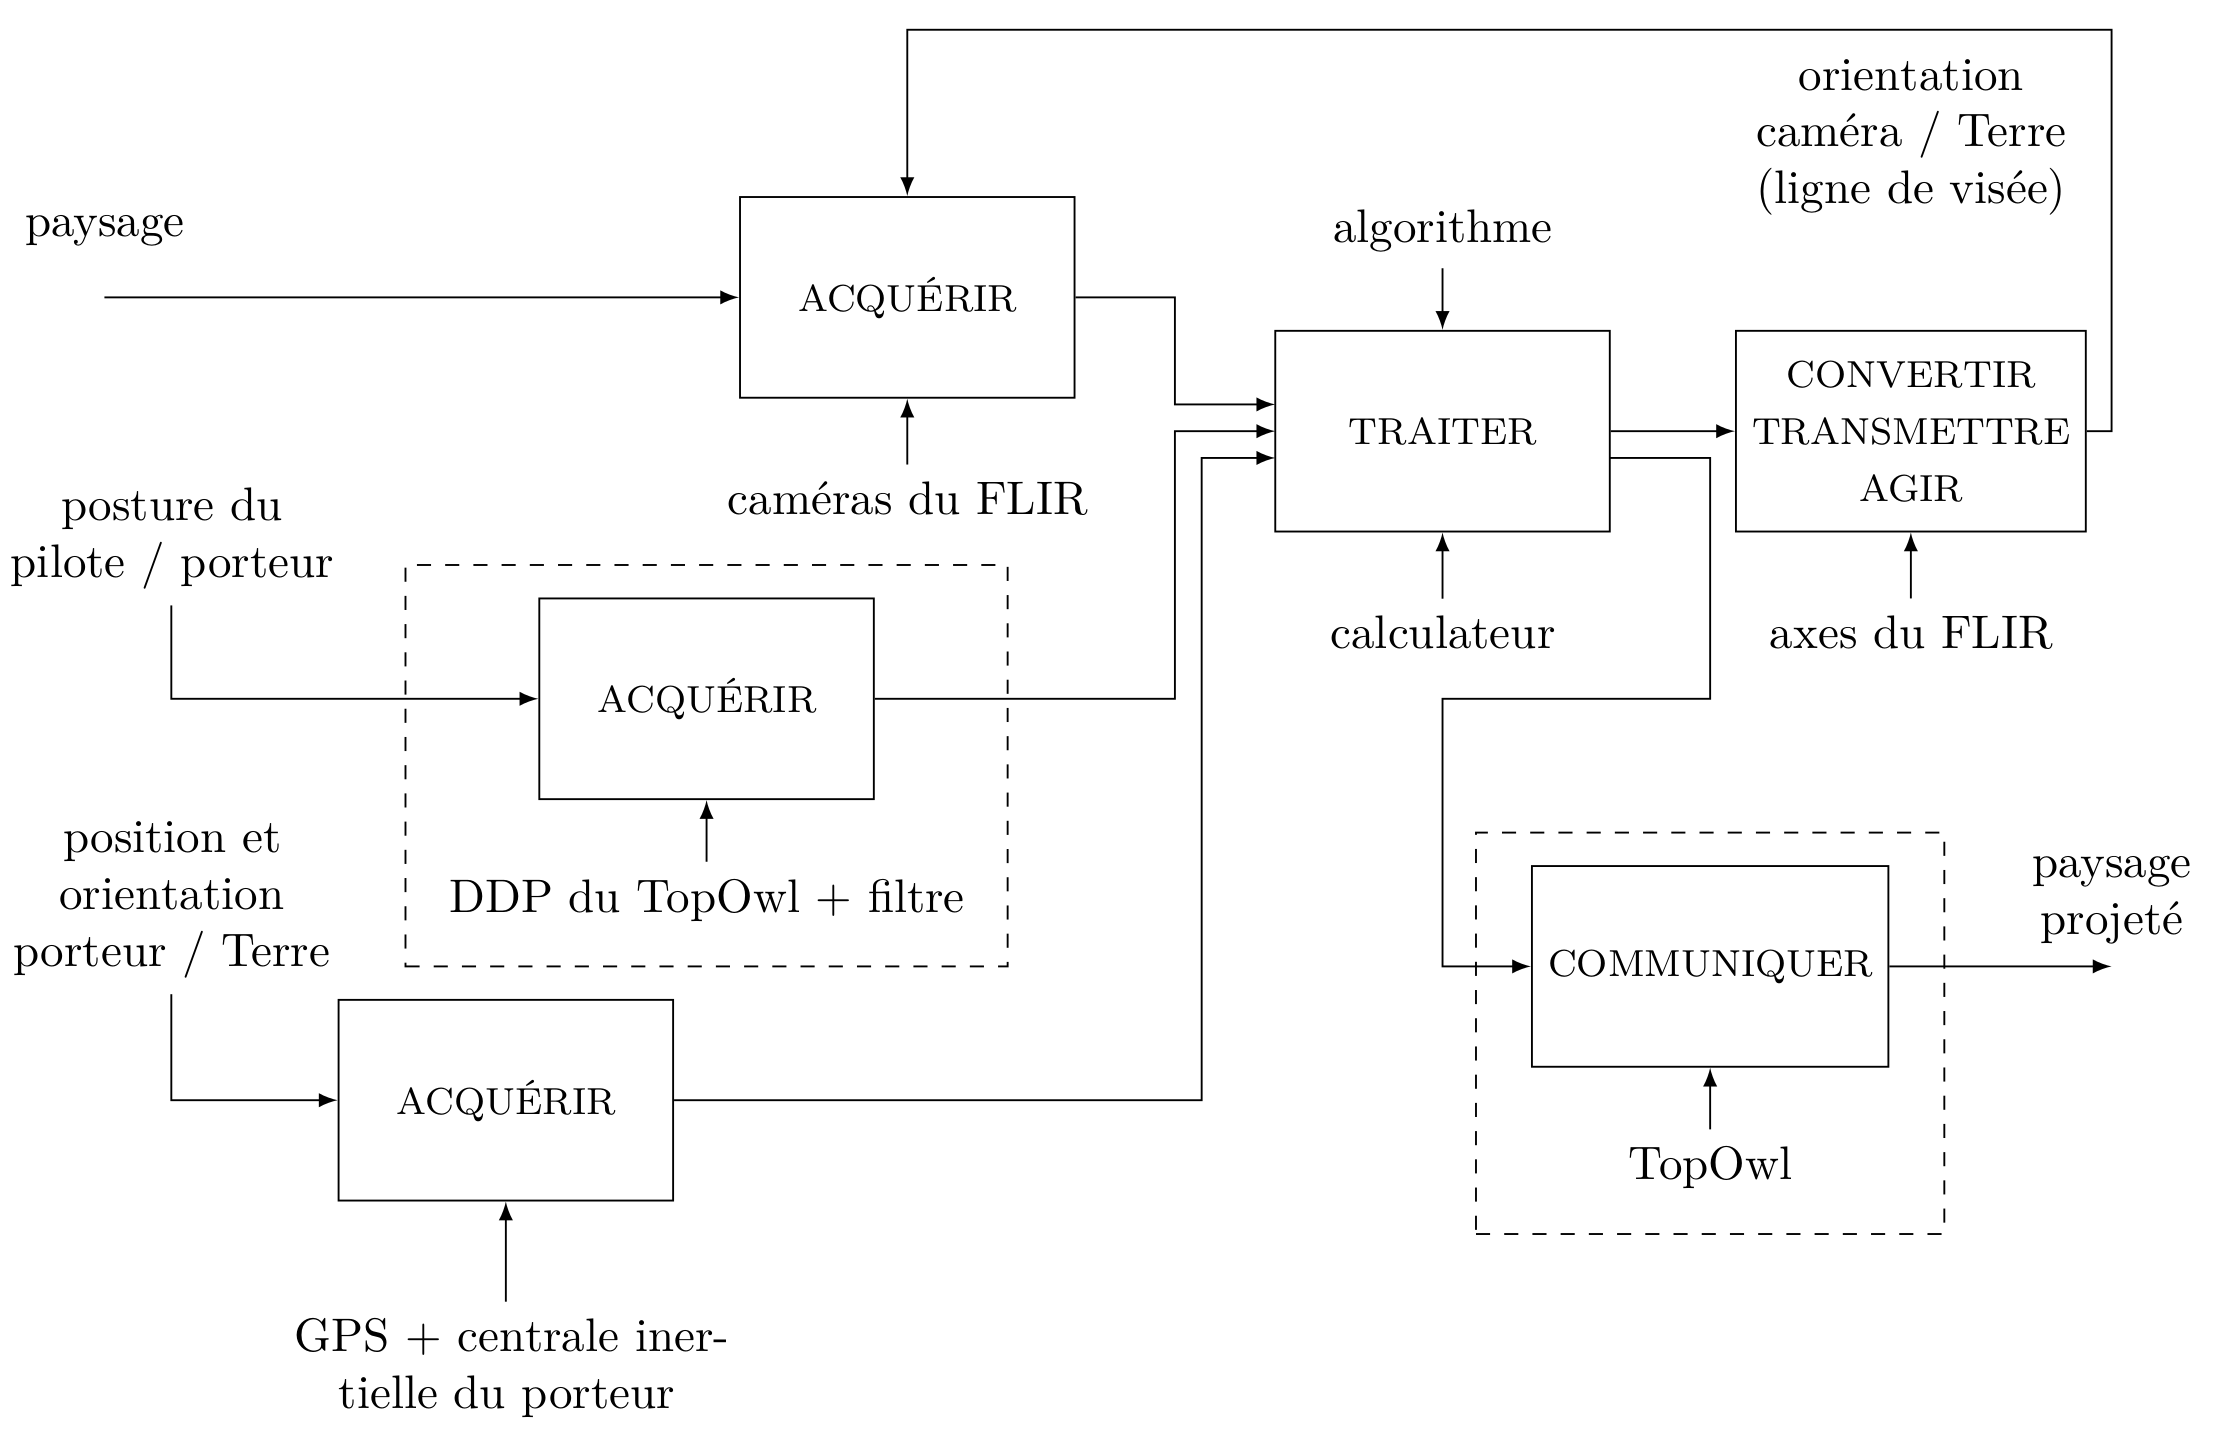
\includegraphics[width=0.7\linewidth]{img/fig05}
\captionof{figure}{\label{fig05}Description structuro-fonctionnelle du système de vision en réalité augmentée}
\end{center}

\question{À l'aide de la description structuro-fonctionnelle de la figure 5, déterminer littéralement et numériquement en fonction des données précédentes le temps maximal disponible pour orienter les caméras du FLIR, noté $t_{disponible}$, qui permet de vérifier l'exigence '1.3'.}

\begin{center}
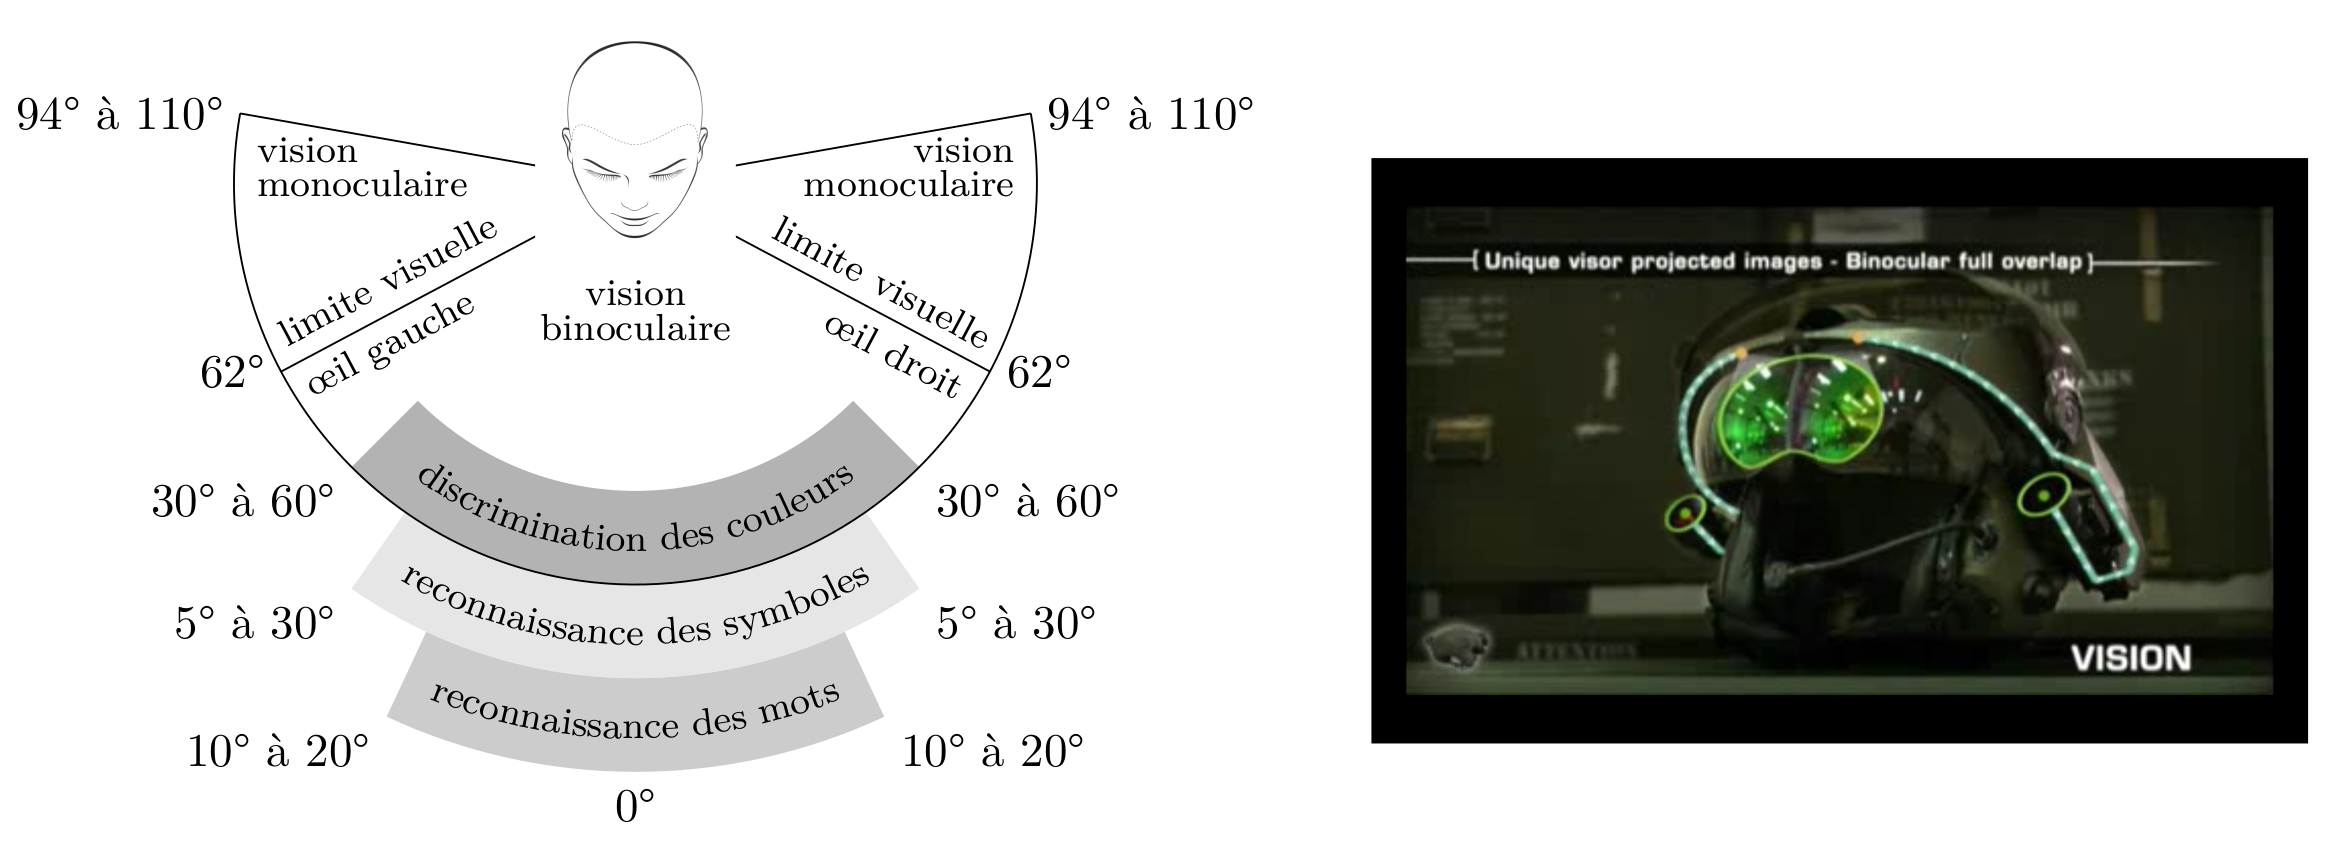
\includegraphics[width=0.7\linewidth]{img/fig06}
\captionof{figure}{\label{fig06}Champ de vision humain et projection des deux images sur la visière}
\end{center}

Le format choisi correspond à une image rectangulaire de 1024 pixels de large et 768 pixels de haut. Cette image est projetée deux fois sur la visière, une projection pour chaque œil du pilote. Les deux projections se chevauchent entièrement (Binocular full overlap). La visière se trouve à 5 cm des yeux du pilote et chaque image est projetée de façon à occuper entièrement le champ de vision le plus large possible permettant la reconnaissance des mots.

\question{Calculer la largeur d'une image couvrant ce champs et placée à 5cm de l'\oe il du pilote. Calculer à partir des informations précédentes et de la figure 6 la largeur d'un pixel (en mm) projeté sur la visière. Conclure quant au respect du critère de résolution d'affichage de l'exigence '1.1'.}

\question{Déterminer l'écart angulaire maximal admissible, exprimé en rad, entre la ligne de visée du pilote et la ligne de visée des caméras qui permet de respecter le critère de précision de l'exigence '1.2'.}

Afin de vérifier les performances du FLIR qui viennent d'être déterminées, et compte tenu de son niveau de complexité élevé, il est nécessaire d'émettre et de valider des hypothèses simplificatrices de modélisation relatives à son comportement.

\section{Architecture du FLIR et hypothèses de modélisation}

\paragraph{Objectif} Vérifier que le choix de l'architecture du FLIR permet de satisfaire les performances établies en partie I. Valider des hypothèses simplificatrices afin de pouvoir évaluer les performances du FLIR.

\subsection{Description et validation de l'architecture du FLIR}

\paragraph{Objectif} Valider le choix de l'architecture du FLIR.

Le FLIR, fixé au porteur, est constitué :
\begin{itemize}
 \item d'un axe motorisé d'azimut orientable en rotation par rapport au porteur autour de l'axe $(P,\overrightarrow{z_P})$,
 \item d'un ensemble de caméras, appelé charge, encastré sur un axe motorisé d'élévation orientable en rotation par rapport à l'axe motorisé d'azimut autour de l'axe $(P,\overrightarrow{y_e})$.
Le modèle cinématique du FLIR et son paramétrage sont donnés sur la figure 7.
\end{itemize}

\begin{center}
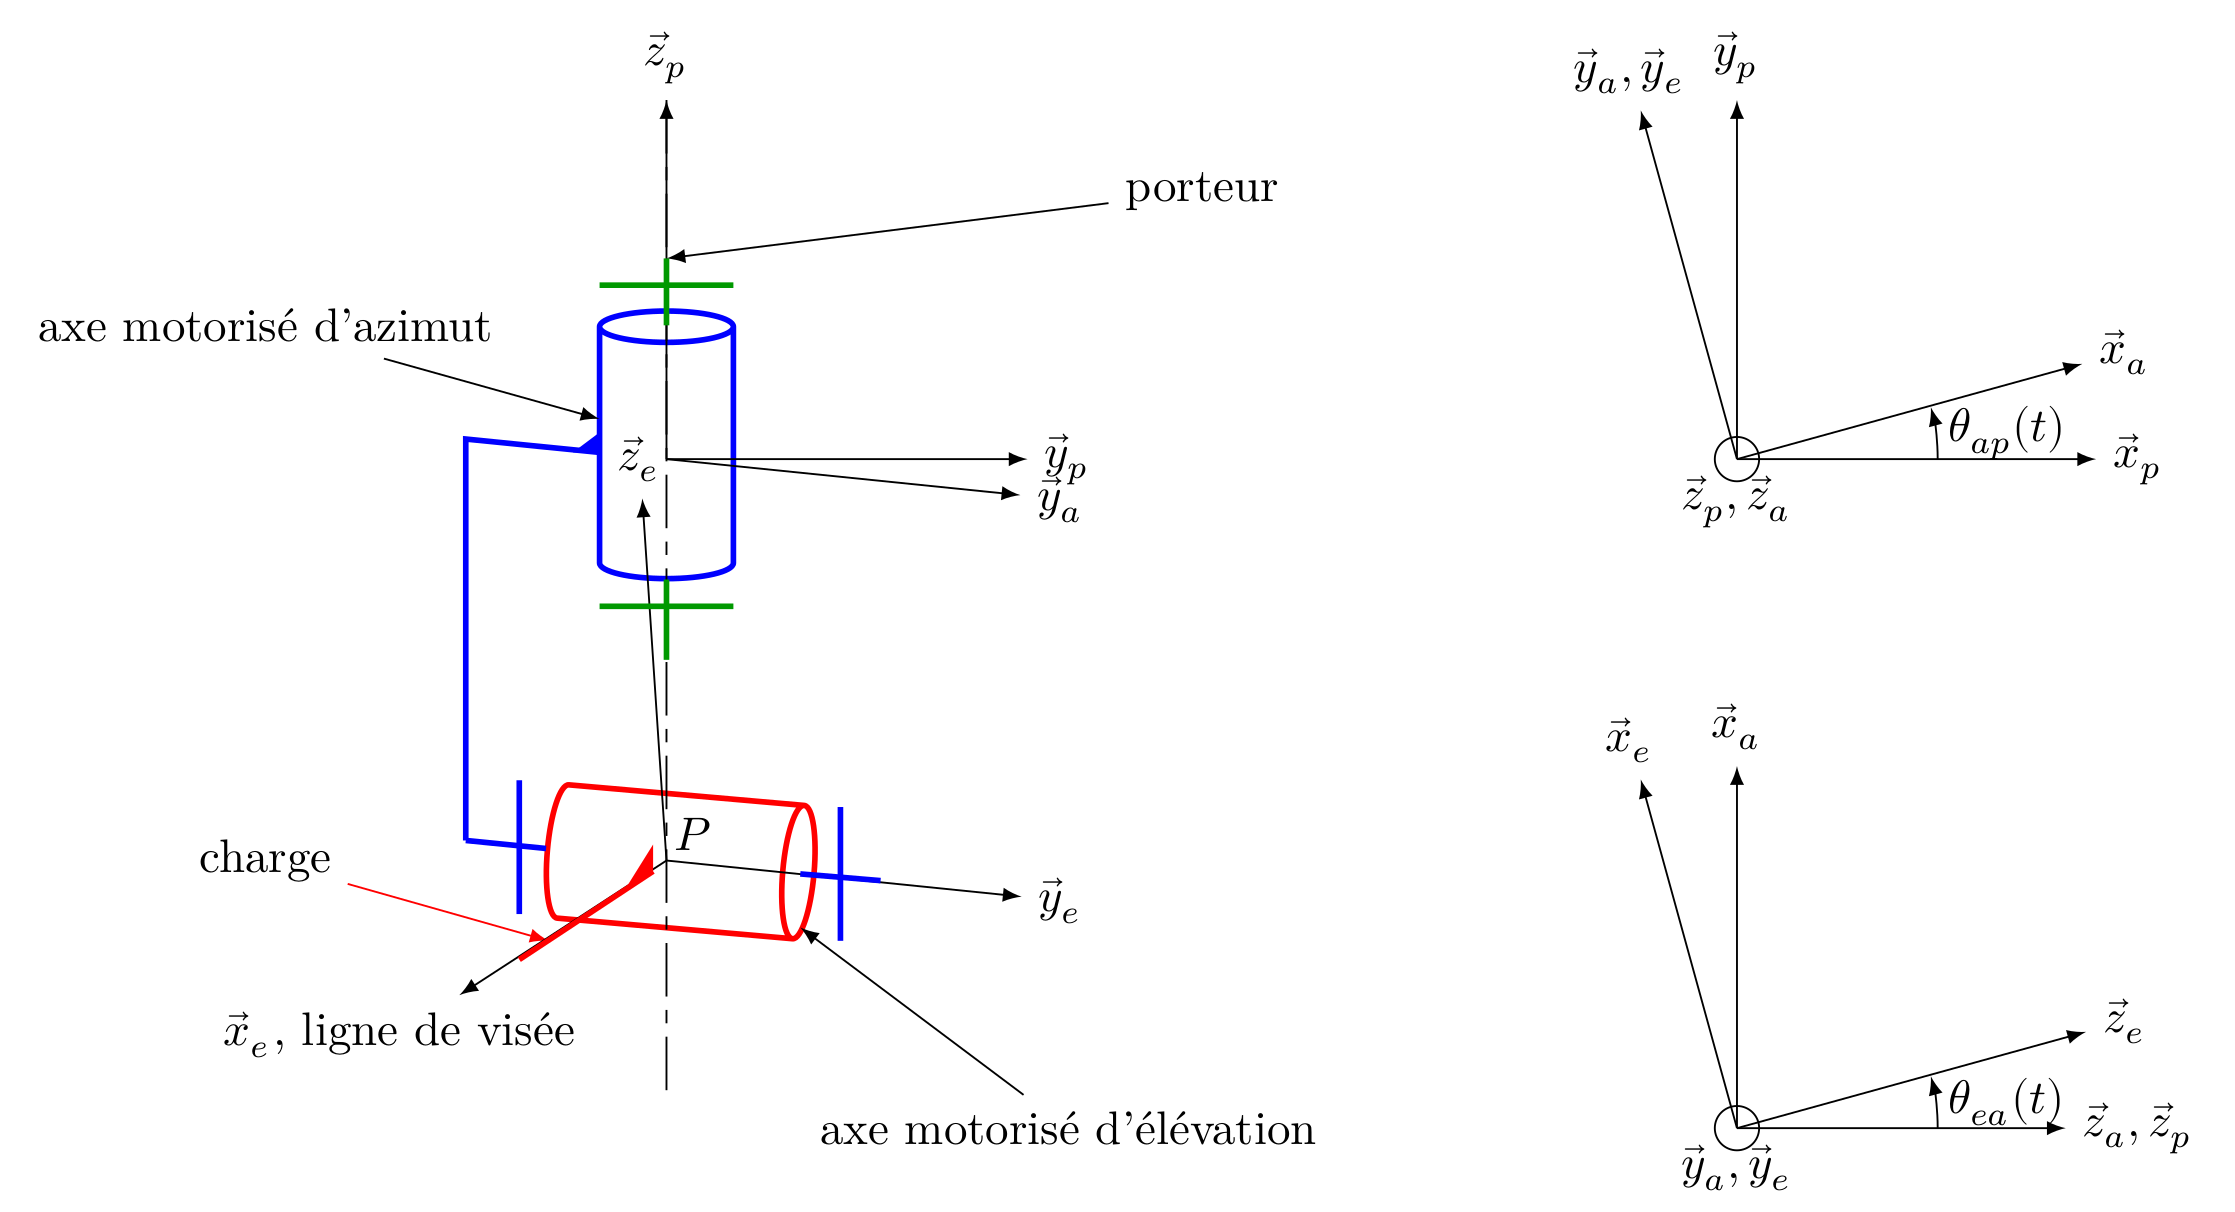
\includegraphics[width=0.9\linewidth]{img/fig07}
\captionof{figure}{\label{fig07}Modèle cinématique global paramétré du FLIR, motorisations enlevées}
\end{center}

Les repères associés aux solides sont les suivants :
\begin{itemize}
 \item $R_a(P,\overrightarrow{x_a},\overrightarrow{y_a},\overrightarrow{z_a})$ pour l'axe motorisé d'azimut,
 \item $R_e(P,\overrightarrow{x_e},\overrightarrow{y_e},\overrightarrow{z_e})$ pour l'ensemble {axe motorisé d'élévation, charge} dont la ligne de visée est portée par $\overrightarrow{x_e}$,
 \item $R_p(P,\overrightarrow{x_p},\overrightarrow{y_p},\overrightarrow{z_p})$ pour le porteur,
 \item $R_0(O_0,\overrightarrow{X_0},\overrightarrow{Y_0},\overrightarrow{Z_0})$ référentiel terrestre non géocentrique, placé à la surface de la Terre au voisinage du porteur avec $Z_0$ vertical ascendant.
\end{itemize}

Dans la suite du sujet, le référentiel $R_0$ est considéré comme galiléen.

\begin{center}
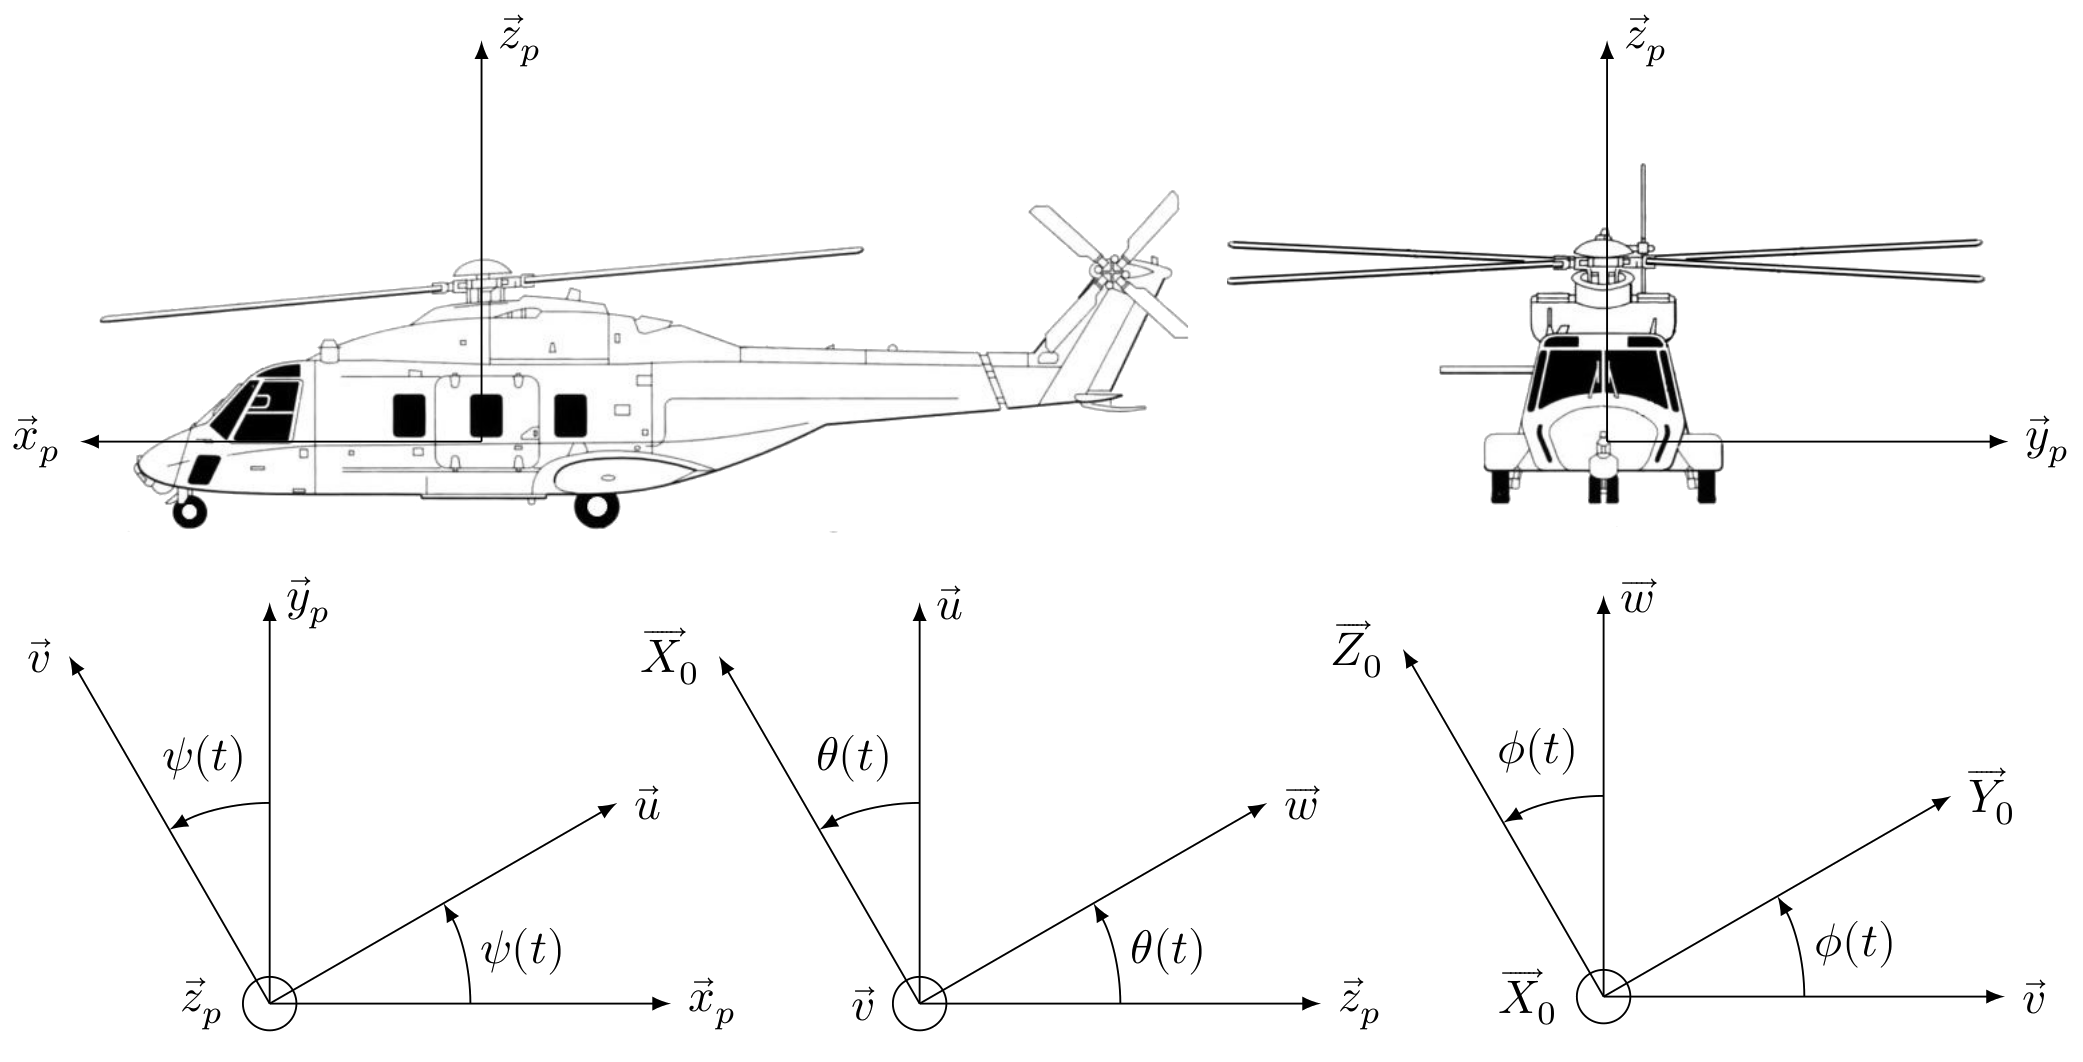
\includegraphics[width=0.8\linewidth]{img/fig08}
\captionof{figure}{\label{fig08}Porteur NH90 et son orientation par rapport au référentiel terrestre}
\end{center}

Le passage du référentiel terrestre $R_0$ au repère du porteur $R_p$ se fait par l'intermédiaire des trois angles de Cardan définis sur la figure 8, avec :
\begin{itemize}
 \item $\phi(t)$ l'angle de roulis,
 \item $\theta(t)$ l'angle de tangage,
 \item $\psi(t)$ l'angle de lacet.
\end{itemize}

\question{Déterminer le torseur cinématique en P, exprimé dans la base $(\overrightarrow{x_a},\overrightarrow{y_a},\overrightarrow{z_a})$ de la liaison équivalente entre le porteur et la charge. En déduire la nature de cette liaison équivalente et préciser ses caractéristiques
géométriques (ex: point, axe, direction, normale,...)}

\medskip

Dans un cas d'utilisation normal, la liaison cinématique entre la tête du pilote et le cockpit est assimilable à une liaison sphérique dont le centre se trouve au milieu de la nuque. Or, le pilote doit avoir une image cohérente à sa vision quelle que soit l'orientation de sa tête par rapport au porteur.

\question{Afin de pouvoir valider la solution technique retenue pour la structure cinématique à deux axes orthogonaux motorisés du FLIR, comparer les mobilités (nombre, type,...) du FLIR et celles de la tête du pilote par rapport au porteur et expliquer quel doit être un des rôles de l'algorithme implanté dans le calculateur.}

\medskip

Le paramétrage de la figure \ref{fig08} a permis décrire les vecteurs de la base $R_0$ dans la base $R_p$. Cela a permis de définir la matrice $M_{rot}$ comme suit:

\begin{center}
$M_{rot}=\left(\begin{array}{ccc}
A & B & C\\
D & E & F\\
G & H & I
\end{array}
\right)$, avec $\left\{\begin{array}{l}
\overrightarrow{X_0}=A.\overrightarrow{x_p}+B.\overrightarrow{y_p}+C.\overrightarrow{z_p} \\
\overrightarrow{Y_0}=D.\overrightarrow{x_p}+E.\overrightarrow{y_p}+F.\overrightarrow{z_p} \\
\overrightarrow{Z_0}=G.\overrightarrow{x_p}+H.\overrightarrow{y_p}+I.\overrightarrow{z_p}
\end{array}\right.$
\end{center}

On pourra montrer que $A=cos\theta.cos\psi$

\question{Déterminer toutes les autres composantes de la matrice $M_{rot}$.}

\subsection{Hypothèses simplificatrice}

\paragraph{Objectif} Valider les hypothèses simplificatrices suivantes :
\begin{itemize}
 \item la commande de l'axe motorisé d'azimut est indépendante des mouvements de l'axe motorisé
d'élévation,
 \item les effets aérodynamiques et la variation de position du centre d'inertie de la charge n'influent pas sur les performances du FLIR.
\end{itemize}

%\subsubsection{Limitation de l'étude à l'axe motorisé d'élévation}
%
%La charge mue par l'axe motorisé d'élévation est essentiellement constituée de caméras et de cartes électroniques associées. Les ingénieurs ont choisi de disposer ces composants de telle sorte que la répartition des masses de cette charge s'approche au mieux de celle d'un cylindre plein et homogène d'axe $(P,\overrightarrow{y_e})$ de la figure 7.
%
%\question{Justifier que le choix de la répartition des composants de la charge, dans le cas du mouvement simultané des deux axes motorisés décrits sur la figure 7, permet de commander l'axe d'azimut indépendamment de l'axe motorisé d'élévation.}
%
%Les résultats d'essais en vol montrent que l'axe qui subit le plus de perturbations est l'axe motorisé d'élévation.
%
%Les commandes des axes d'élévation et d'azimut étant indépendantes l'une de l'autre, la suite de l'étude se limitera uniquement à l'axe motorisé d'élévation.

\subsubsection{Rigidité de la structure à double étage de l'axe motorisé d'élévation et influence des perturbations aérodynamiques}

Afin de limiter l'influence des vibrations du porteur sur la ligne de visée et augmenter la précision de son orientation, les ingénieurs ont choisi de décomposer l'axe motorisé d'élévation en deux étages (voir figures 9 et 10).

Le premier étage, appelé étage gros d'élévation (ge), est en prise directe avec l'air et est donc soumis aux effets aérodynamiques lors des mouvements du porteur. L'étage gros d'élévation est lui même en liaison pivot, d'axe $(P,\overrightarrow{y_e})$, avec l'axe motorisé d'azimut.

Le second, appelé étage fin d'élévation (fe), est protégé des effets aérodynamiques grâce au carter sphérique solidaire de l'étage gros. Cet étage est en liaison pivot, d'axe $(P,\overrightarrow{y_e})$, avec l'étage gros d'élévation. L'inertie des Figure 9 Intérieur du FLIR, vue des optiques des éléments déplacés par l'étage fin d'élévation est plus faible caméras liées à l'étage fin d'élévation que celle de l'étage gros d'élévation et les choix de guidage
et de motorisation permettent d'atteindre des accélérations et des vitesses élevées. Cependant, l'amplitude du mouvement de l'étage fin est limitée.

\begin{center}
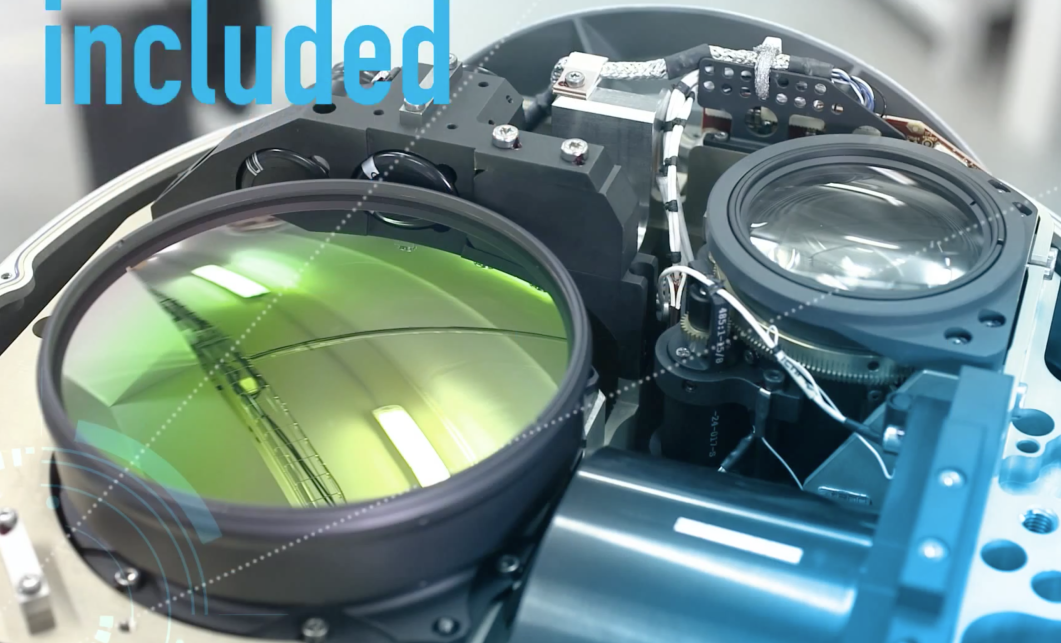
\includegraphics[width=0.5\linewidth]{img/fig09}
\captionof{figure}{\label{fig09}Intérieur du FLIR, vue des optiques des caméras liées à l'étage fin d'élévation}
\end{center}

\begin{center}
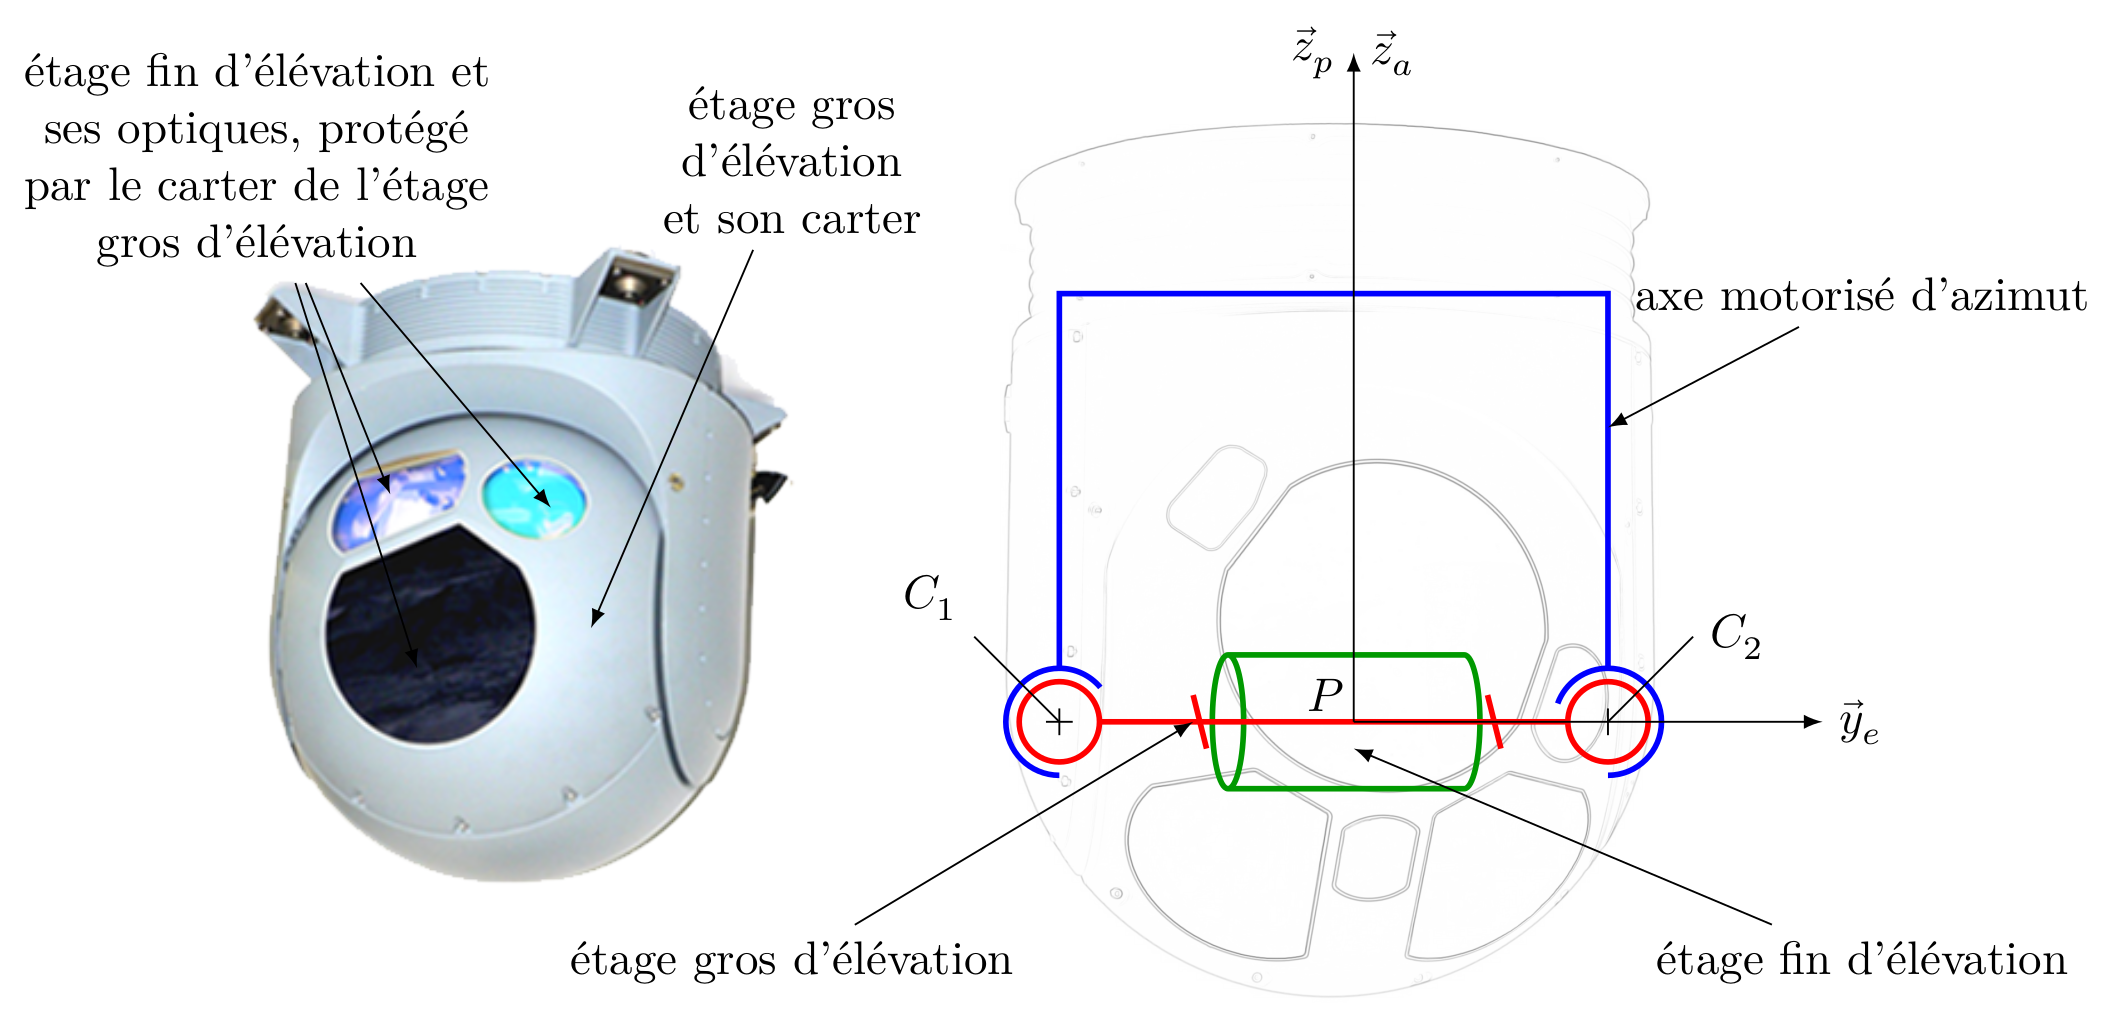
\includegraphics[width=0.8\linewidth]{img/fig10}
\captionof{figure}{\label{fig10}FLIR et modèle cinématique de l'axe motorisé d'élévation}
\end{center}

Le guidage en rotation entre l'étage gros d'élévation et l'axe motorisé d'azimut est réalisé à l'aide de deux composants à éléments roulants modélisables par des liaisons sphériques de centre $C_1$ et $C_2$.

\question{À l'aide de la figure 10, déterminer le degré d'hyperstatisme du modèle du guidage en rotation entre l'axe motorisé d'azimut et l'étage gros d'élévation. Lister deux avantages et un inconvénient de ce guidage, puis conclure quant à sa pertinence vis-à-vis de la précision de l'orientation de la ligne de visée souhaitée.}

\subsubsection{Influence du déport de masse lié à la variation de position des optiques}

Le déplacement des optiques (zoom) en translation rectiligne suivant $\overrightarrow{x_e}$ par rapport à l'étage fin d'élévation rend la géométrie de ce dernier variable et son centre d'inertie ne se situe pas exactement sur l'axe de rotation $(P,\overrightarrow{y_e})$ de l'étage fin d'élévation par rapport à l'étage gros d'élévation.

L'étage fin d'élévation est modélisé par l'ensemble des deux solides suivants (voir figure 12) :
\begin{itemize}
 \item un disque plein et homogène d'axe $(P_0,\overrightarrow{x_e})$ de masse $m_o$, de rayon $r_o$ et de centre de gravité $P_o$, modélisant les optiques mobiles de l'étage fin d'élévation,
 \item un cylindre plein et homogène d'axe $(P,\overrightarrow{y_e})$ de masse $m_{cyl}$, de rayon $r_{cyl}$, de hauteur $h_{cyl}$ et de centre de gravité $P$, modélisant le reste des éléments de l'étage fin d'élévation.
\end{itemize}

Dans la suite, ces deux solides sont supposés être en liaison complète, c'est-à-dire que la distance $d$, telle que $\overrightarrow{PP_o}=d.\overrightarrow{x_e}$, est constante.

\begin{center}
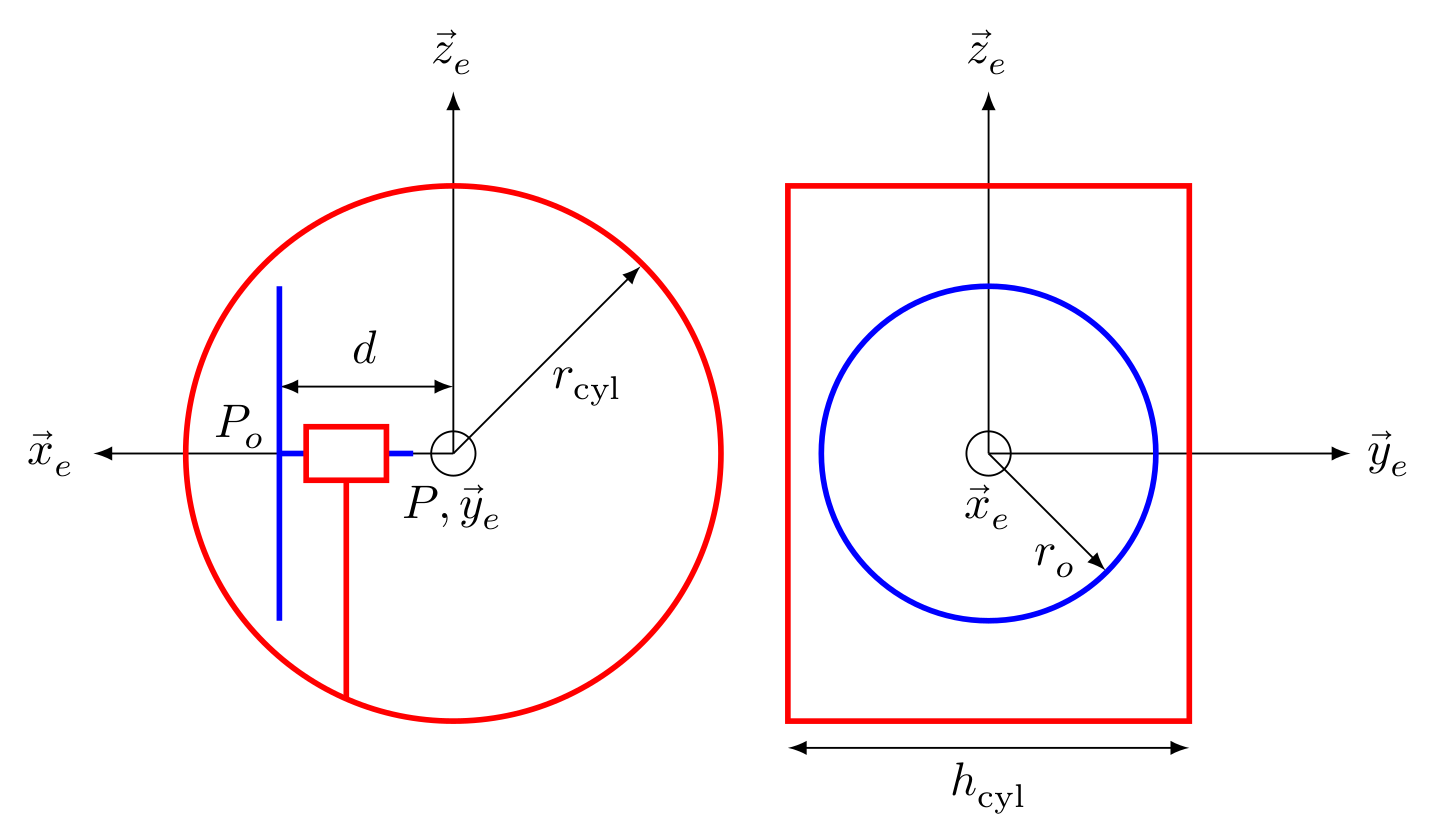
\includegraphics[width=0.7\linewidth]{img/fig11}
\captionof{figure}{\label{fig11}Modélisation de la géométrie des masses de l'étage fin d'élévation}
\end{center}

L'étage fin d'élévation est noté $fe$, sa masse est égale à $m_{fe}=m_{cyl}+m_o$, son centre d'inertie est noté $G_{fe}$. Une étude de dynamique a permis de montrer que $\overrightarrow{PG_{fe}}=\frac{m_o.d}{m_o+m_{cyl}}.\overrightarrow{x_e}$.

Des mesures à bord du NH90 ont montré que la phase de vol la plus pénalisante, c'est-à-dire celle qui perturbe le plus la ligne de visée du FLIR, est l'ascension verticale du porteur. Dans cette phase, il est possible d'effectuer les hypothèses suivantes :
\begin{itemize}
 \item les angles $\psi(t)$, $\theta(t)$ et $\phi(t)$ sont constants et nuls,
 \item $\theta_{ap}(t)$ = 0,
 \item $\overrightarrow{z_p}=\overrightarrow{z_a}=\overrightarrow{Z_0}$ vertical ascendant, $\overrightarrow{y_p}=\overrightarrow{y_a}=\overrightarrow{Y_0}$ et $\overrightarrow{x_p}=\overrightarrow{x_a}=\overrightarrow{X_0}$,
 \item l'étage fin d'élévation est en mouvement par rapport à l'étage gros d'élévation,
 \item la ligne de visée est définie par l'orientation $\theta_{e0}(t)$ de l'étage fin d'élévation par rapport à $R_0$. Dans cette étude, $\theta_{e0}(t)=\theta_{ea}(t)$,
 \item $R_0$ est galiléen,
 \item le couple moteur sur l'étage fin d'élévation est noté $C_m(t)$,
 \item la liaison pivot entre l'étage fin d'élévation et l'étage gros d'élévation est supposée parfaite.
\end{itemize}

La vitesse d'ascension verticale du porteur est notée $\overrightarrow{V_{P\in porteur/Ro}}=v(t).\overrightarrow{Z_0}$ et son accélération est notée $\overrightarrow{\Gamma_{P\in porteur/Ro}}=\gamma(t).\overrightarrow{Z_0}$

Les dérivées d'un paramètre $x(t)$ par rapport au temps seront notées: $\dot{x}(t)=\frac{dx(t)}{dt}$ et $\ddot{x}(t)=\frac{d^2x(t)}{dt^2}$.

\question{Exprimer $\overrightarrow{V_{G_{fe}\in fe/Ro}}$ dans le repère $R_0$, vecteur vitesse du point $G_{fe}$, centre d'inertie de l'étage fin d'élévation dans son mouvement par rapport à $R_0$, en fonction de $v(t)$, $m_{cyl}$, $m_o$, $d$, $\theta_{e0}(t)$ et $\dot{\theta}_{e0}(t)$.}

\question{En déduire $\overrightarrow{\Gamma_{G_{fe}\in fe/Ro}}$ dans le repère $R_0$, vecteur accélération du point $G_{fe}$, centre d'inertie de l'étage fin d'élévation dans son mouvement par rapport à $R_0$, en fonction de $\gamma(t)$, $m_{cyl}$, $m_o$, $d$, $\theta_{e0}(t)$, $\dot{\theta}_{e0}(t)$et $\ddot{\theta}_{e0}(t)$.}

\section{Conception de la commande de l'axe motorisé d'élévation à partir des performances attendues et vérification des performances simulées du FLIR}

\paragraph{Objectif} Modéliser l'asservissement de l'axe motorisé d'élévation, concevoir sa commande puis vérifier ses performances simulées vis-à-vis du cahier des charges donné figure 13.

\begin{center}
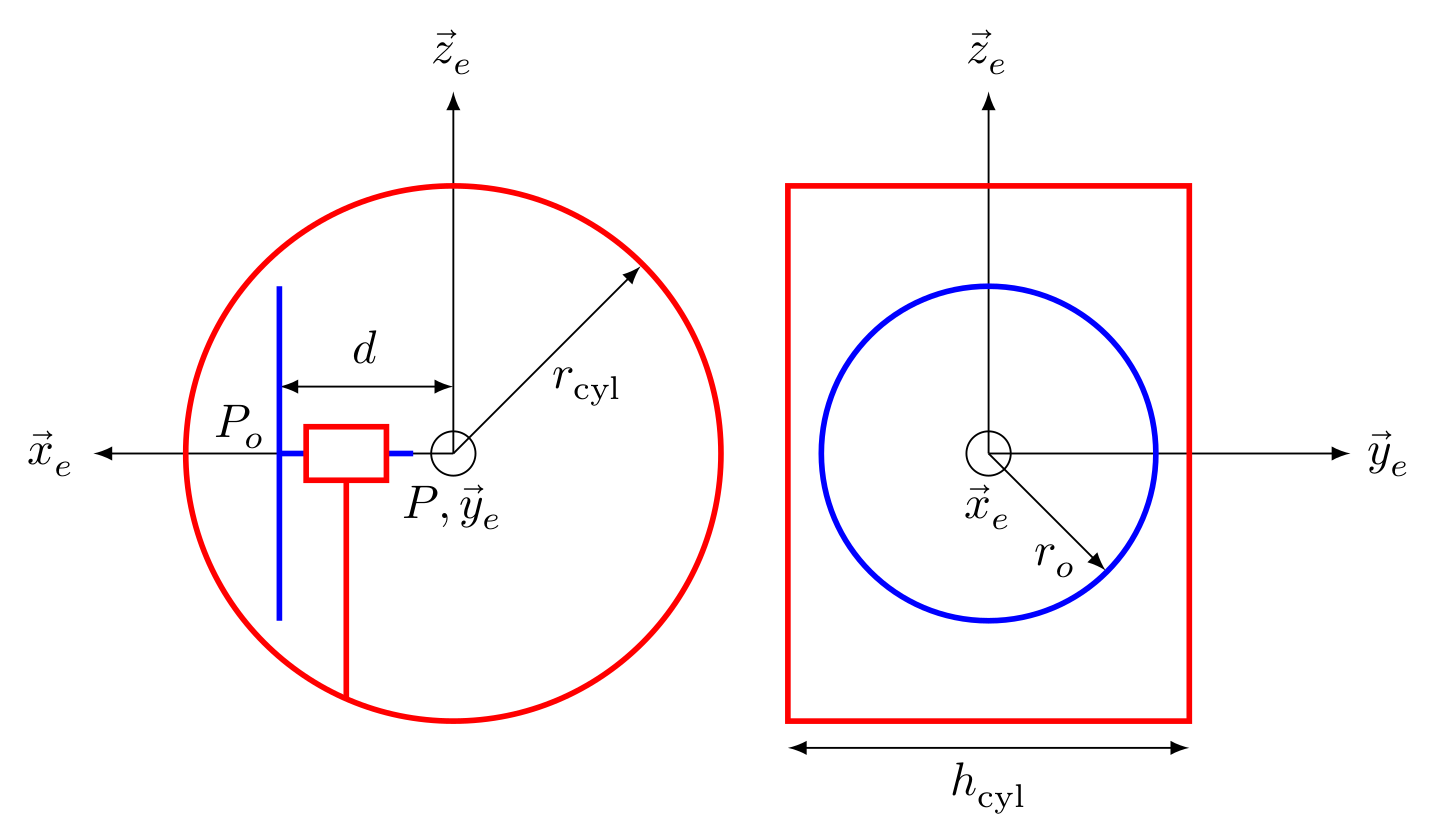
\includegraphics[width=0.7\linewidth]{img/fig11}
\captionof{figure}{\label{fig12}DIAGRAMME DES EXIGENCES A FAIRE}
\end{center}

\subsection{Modélisation de l'asservissement de l'étage fin d'élévation et conception de sa commande}

\paragraph{Objectif} En s'appuyant sur les hypothèses validées en partie II, compléter la modélisation de l'asservissement de l'étage fin d'élévation et ajuster un correcteur qui lui permette d'atteindre les performances attendues.

\subsubsection{Modélisation de l'asservissement de l'étage fin d'élévation}

Un gyromètre est placé directement sur l'étage fin d'élévation et permet de mesurer $\omega_{fe0\  mes}(t)$, taux de rotation de l'étage fin d'élévation par rapport au référentiel galiléen $R_0$. Les ingénieurs ont donc choisi d'asservir l'étage fin d'élévation en vitesse angulaire afin d'utiliser directement la mesure du gyromètre.

La direction de la ligne de visée est paramétrée par rapport au référentiel galiléen $R_0$ par l'angle $\theta_{fe0}(t)=\theta_{e0}(t)$.

Sont donnés les éléments suivants :
\begin{itemize}
 \item $\dot{\theta}_{fe0}(t)=\omega_{fe0}(t)=\overrightarrow{\Omega_{fe/R_0}}.\overrightarrow{y_e}$ où $\overrightarrow{\Omega_{fe/R_0}}$ est le vecteur taux de rotation de l'étage fin d'élévation ($fe$) dans son mouvement par rapport au référentiel terrestre $R_0$,
 \item le comportement du gyromètre, placé directement sur l'étage fin d'élévation, peut être modélisé par un premier ordre de gain unitaire et de bande passante à -3dB égale à 100 Hz,
 \item l'étage fin d'élévation ($fe$) est actionné par un moteur électrique linéaire comme indiqué sur la figure 14, dont la tige est en liaison sphérique en A avec l'étage fin d'élévation et le carter en liaison sphérique en B avec l'étage gros d'élévation,
 \item l'isolement de la tige seule du moteur électrique linéaire permet de modéliser son action mécanique de liaison en A sur l'étage fin d'élévation par un glisseur au point A de résultante $F_{mot}(t).\overrightarrow{u}$,
 \item l'étage fin d'élévation ($fe$) est en liaison pivot d'axe (P,$\overrightarrow{y_e}$) avec l'étage gros d'élévation ($ge$),
 \item $\overrightarrow{AP}=r.\overrightarrow{x_e}$, avec $r=10cm$,
 \item $\lambda(t)$ paramètre la position de la tige par rapport au carter du moteur électrique linéaire tel que $\overrightarrow{BA}=\lambda(t).\overrightarrow{u}$.
\end{itemize}

Le choix de la motorisation de l'étage fin d'élévation permet d'atteindre des accélérations importantes mais l'amplitude du mouvement de l'étage fin d'élévation ($fe$) par rapport à l'étage gros d'élévation ($ge$) est limitée à l'intervalle [-5°, +5°]. Il est donc nécessaire d'orienter également l'étage gros d'élévation (ge) grâce au moteur à courant continu de la figure 14.

Hypothèses :
\begin{itemize}
 \item 0 par rapport au référentiel galiléen R 0,
 \item le porteur est en translation suivant Z,
 \item l'étage gros d'élévation ($ge$) est fixe par rapport au porteur, c'est-à-dire que $\dot{\theta}_{ge0}(t)=\omega_{ge0}(t)=0$ et $\dot{\theta}_{ge0}(t)=\alpha$, avec $\alpha$ un angle constant,
 \item l'orientation de l'étage gros d'élévation ($ge$) est telle que $\overrightarrow{u}\approx \overrightarrow{z_e}$,
 \item la liaison pivot entre l'étage fin d'élévation ($fe$) et l'étage gros d'élévation ($ge$) est parfaite,
% \item le moment d'inertie de l'étage fin d'élévation ($fe$) autour de l'axe ($P,\overrightarrow{y_e}$) est noté $B_{fe}=0,1kg.m^2$,
 \item  le centre de gravité de l'étage fin d'élévation ($fe$) est considéré en P, c'est-à-dire que $P=G_{fe}$ (voir figure 12),
 \item $\overrightarrow{V_{A\in fe/ge}}= v_{tige}(t).\overrightarrow{z_e}$, avec $\dot{\lambda}(t)= v_{tige}(t)$ et $\overrightarrow{u}\approx \overrightarrow{z_e}$,
 \item $\overrightarrow{V_{A\in ge/R_0}}=\overrightarrow{V_{P\in ge/R_0}}=v(t).\overrightarrow{Z_0}$.
\end{itemize}

\begin{center}
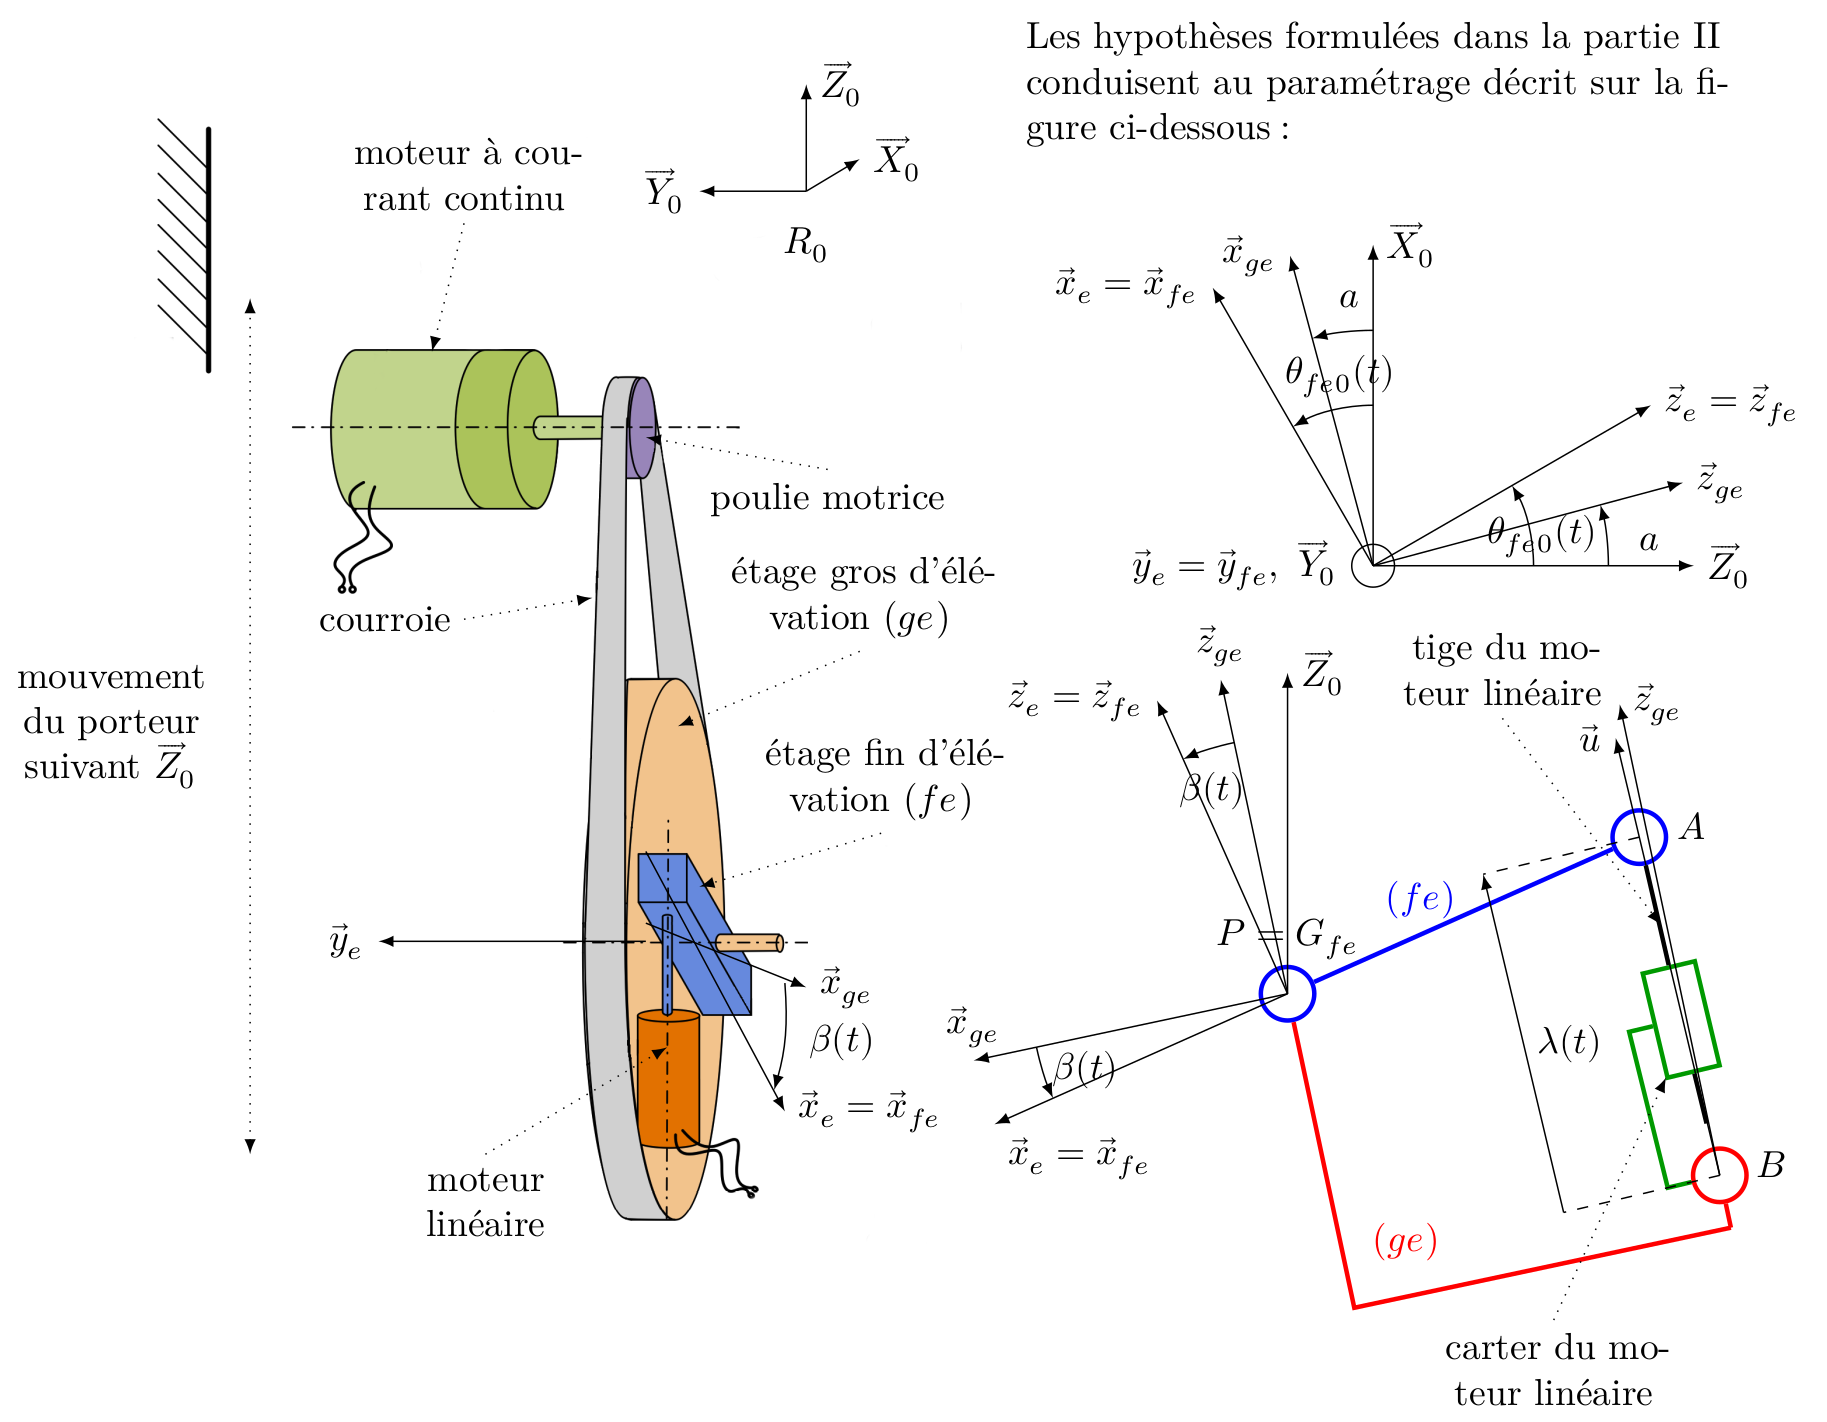
\includegraphics[width=0.9\linewidth]{img/fig12}
\captionof{figure}{\label{fig13}Structure et paramétrage des étages fin et gros de l'axe motorisé d'élévation}
\end{center}

\question{Exprimer le vecteur vitesse $\overrightarrow{V_{A\in fe/R_0}}$ en fonction de $r$, $v(t)$ et $\dot{\theta}_{fe0}(t)$.}

Une étude dynamique a permis d'obtenir l'équation du mouvement suivante: $B_{fe}.\ddot\theta_{feo}(t)=r.F_{mot}(t)$.

Dans la suite du sujet, le passage dans le domaine symbolique de Laplace est noté de la façon suivante : $F(p)$ est la transformée de Laplace de la fonction $f(t)$, avec $p$ la variable de Laplace. Les conditions de Heaviside sont vérifiées, c'est-à-dire que les valeurs initiales des fonctions temporelles sont nulles.

\question{A partir de l'équation du mouvement précédente, exprimer littéralement la fonction de transfert $\frac{\Omega_{fe0}(p)}{F_{mot}(p)}$ de la figure \ref{fig14} et en déduire les expressions de $M_{eq}$ et $K_1$. Effectuer les applications numériques.}

On rappelle que le gyromètre, placé directement sur l'étage fin d'élévation, permet de mesurer $\omega_{fe0\ mes}(t)$. Son comportement peut être modélisé par un premier ordre de la forme
$\frac{1}{1+\tau_{gyro}.p}$ et de bande passante à -3 dB égale à 100 Hz.

\question{Calculer la valeur numérique de $\tau_{gyro}$.}

Le modèle d'asservissement de l'étage fin d'élévation étant établi, il est alors possible de concevoir sa commande.

\subsubsection{Conception de la commande de l'étage fin d'élévation}

Les performances de l'étage fin d'élévation ont été déterminées à partir des performances du FLIR établies en partie I. Elles sont données dans le tableau de la figure 15.

La consigne de vitesse $\dot{\theta}_{fe0\ cons}(t)=\omega_{fe0\ cons}(t)$ est établie par rapport au référentiel galiléen $R_0$. Elle est calculée à partir de la détection de posture (DDP du casque TopOwl) de la tête du pilote et des informations d'orientation du porteur par rapport au référentiel terrestre $R_0$ obtenues par la centrale inertielle du porteur.

\begin{center}
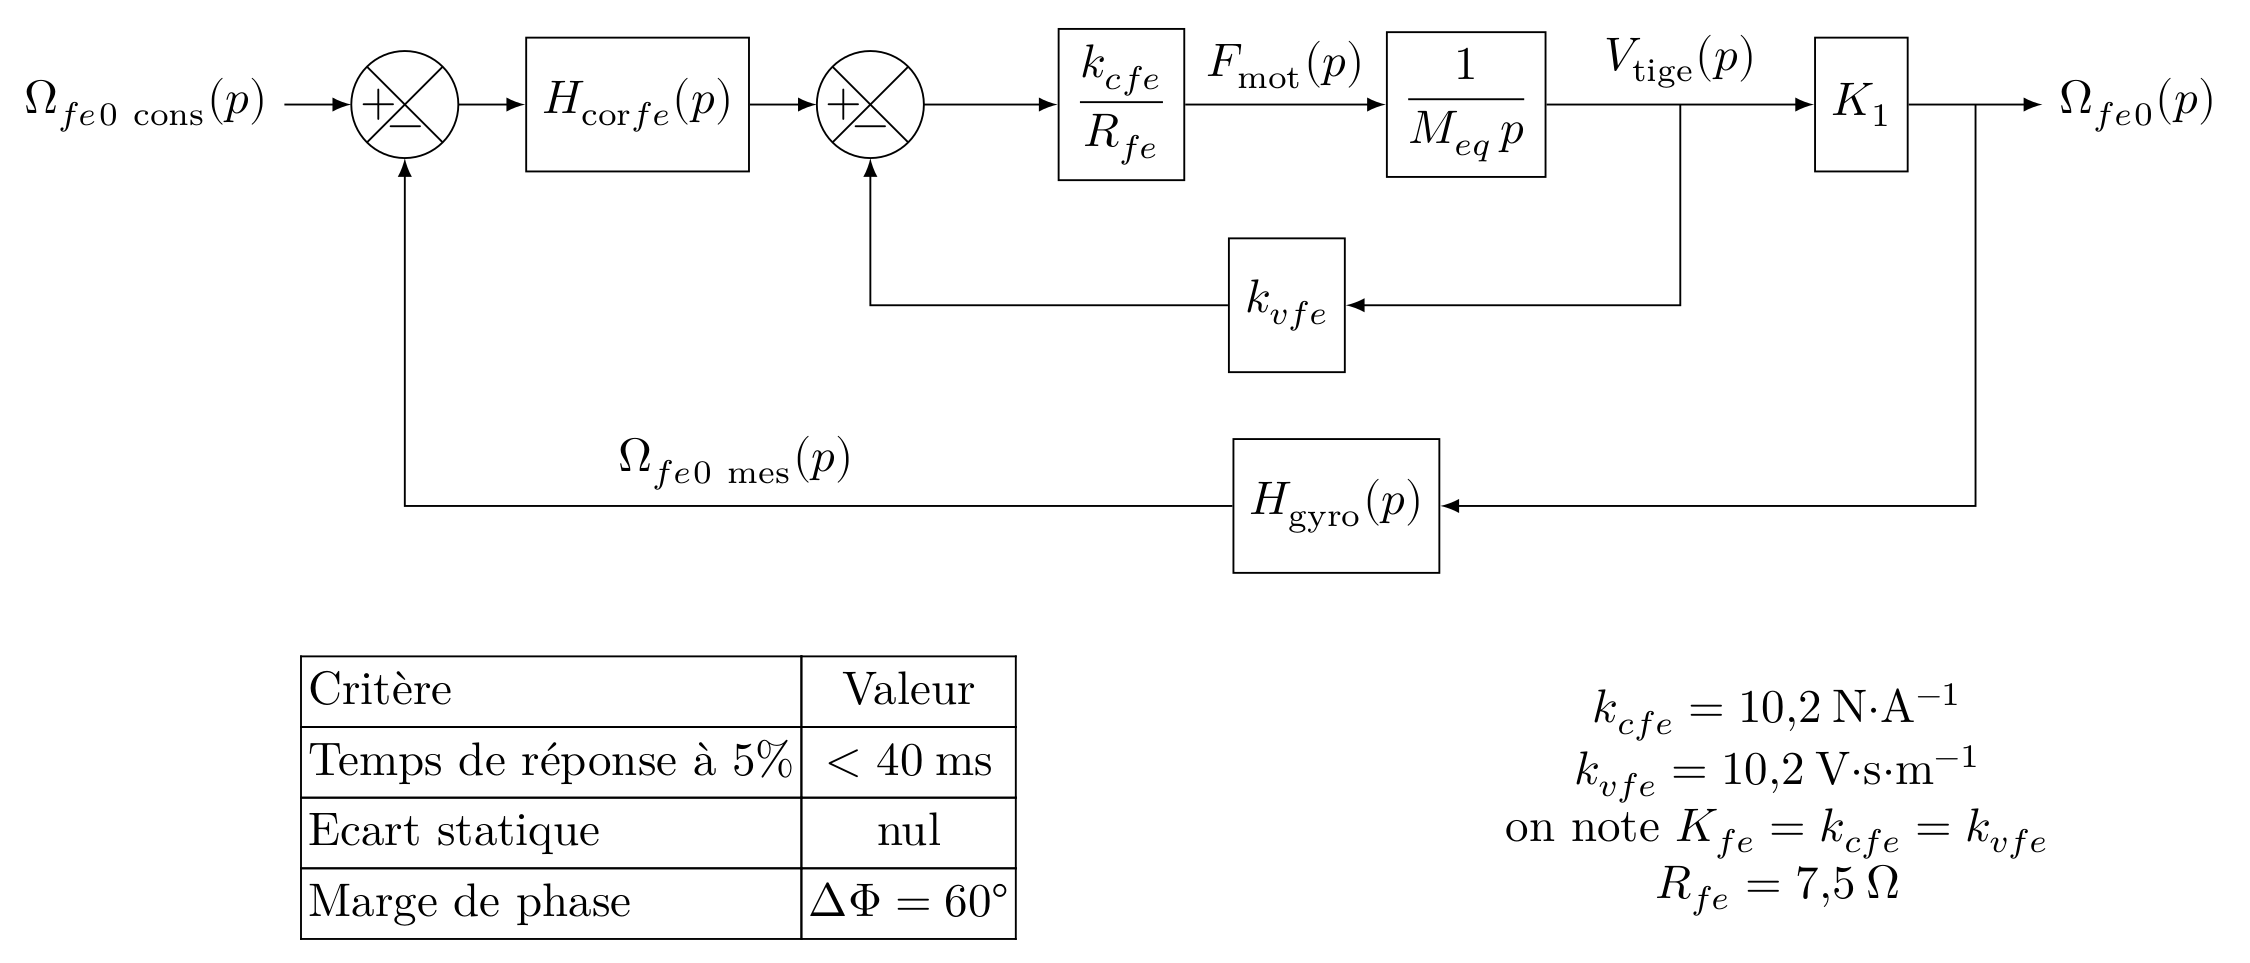
\includegraphics[width=0.9\linewidth]{img/fig13}
\captionof{figure}{\label{fig14}Modèle d'asservissement de l'étage fin d'élévation et performances attendues}
\end{center}

Dans un premier temps, l'asservissement de vitesse n'est pas corrigé, c'est-à-dire que $H_{cor\ fe} (p)=1$.

\question{Exprimer littéralement et sous forme canonique la fonction de transfert $H_{fe1}(p)=\frac{\Omega_{fe0}(p)}{\Omega_{fe0\ cons}(p)}$, en fonction de $K_1$, $\tau_{gyro}$, $M_{eq}$, $K_{fe}$ et $R_{fe}$.}

Compte tenu des temps de réponse à observer, on montre que $H_{fe1}(p)$ peut se mettre sous la forme simplifiée suivante :
\begin{center}
$H_{fe1}(p)=\frac{0,5}{1+3,65.10^{-1}.p+6.10^{-4}.p^2}$
\end{center}

Remarque: On pourra approximer $\sqrt{6}=2.5$.

\question{En utilisant l'abaque de la figure \ref{fig15}, déterminer le temps de réponse à 5\% et l'écart statique de l'asservissement en vitesse de l'étage fin d'élévation en réponse à un échelon de vitesse unitaire. Conclure sur le respect des performances en rapidité et en précision données sur la figure 15.}

\begin{center}
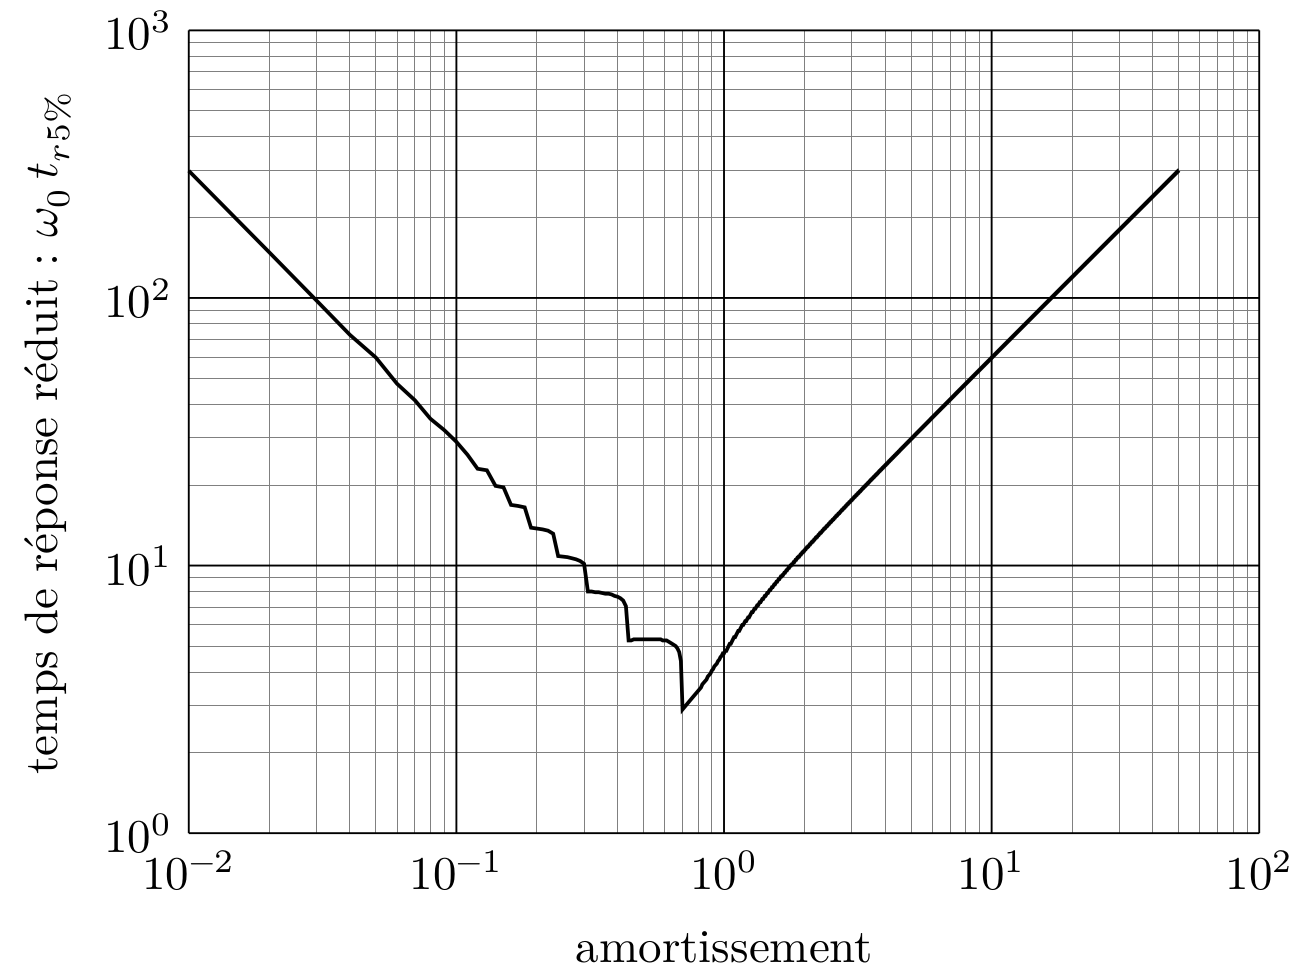
\includegraphics[width=0.7\linewidth]{img/fig14}
\captionof{figure}{\label{fig15}Abaque des temps de réponse réduit}
\end{center}

On propose d'utiliser un correcteur proportionnel intégral de la forme $H_{cor\ fe}(p)=K_{pfe}.\left(1+\frac{1}{T_{ife}.p}\right)$. La fonction de transfert en boucle ouverte de l'asservissement en vitesse de l'étage fin d'élévation devient alors

\begin{center}
$H_{BOfe}(p)=K_{pfe}.\left(1+\frac{1}{T_{ife}.p}\right).\frac{1}{1+0,75.p}.\frac{1}{1+1,6.10^{-3}.p}$
\end{center}

\question{Montrer que l'on peut écrire la fonction de transfert $H_{BOfe}(p)$ comme suit:
\begin{center}
$H_{BOfe}(p)=\frac{K_{pfe}}{T_{ife}.p}.\frac{1+T_{ife}.p}{1}.\frac{1}{1+0,75.p}.\frac{1}{1+1,6.10^{-3}.p}$
\end{center}
}

\question{Tracer sur le document réponse, les tracés asymptotiques des diagrammes de Bode de la fonction $\frac{1}{1+0,75.p}$.}

\question{Tracer sur le document réponse, les tracés asymptotiques des diagrammes de Bode de la fonction $\frac{1+T_{ife}.p}{1}$ en prenant $T_{ife}=0,01s$ pour commencer.}

\question{Tracer alors sur le document réponse, les tracés asymptotiques des diagrammes de Bode de la fonction $\frac{1}{1+0,75.p}.\frac{1+T_{ife}.p}{1}$ en prenant toujours $T_{ife}=0,01s$.}

La figure du document réponse pour la question \ref{19} correspond aux tracés des diagrammes de Bode réels de $H_{BOfe}(j.\omega)$.

\question{Sur cette même figure du document réponse, tracer le diagramme de phase asymptotique de $H_{BOfe}(j.\omega)$ (Bode).}

\question{En déduire la valeur réelle de $T_{ife}$ et de $K_{pfe}$}.

%
%La lecture du tracé réel de la phase met en évidence un maximum à la pulsation $\omega_{max}$ telle que $\omega_{max}\in [1/T_{ife}:600] rad.s^{-1}$.
%
%\question{En supposant que le tracé réel semi-logarithmique de la phase est symétrique autour de $\omega_{max}$, calculer la valeur de $T_{ife}$ comprise dans la décade $[0,01s:0,1s]$ qui permet de régler ce maximum à $-120\textdegree$.}
%
%\question{Pour le réglage de $T_{ife}$ calculé à la question 19 avec $K_{pfe}=1$ et à partir des tracés réels du document réponse, calculer la valeur de $K_{pfe}$ qui permet de respecter le critère de marge de phase du tableau de la figure 15.}

Le modèle est complété en utilisant les réglages déterminés précédemment pour $K_{pfe}$ et $T_{ife}$. Afin de prendre en compte les caractéristiques du moteur linéaire, une saturation d'alimentation du moteur st ajoutée ainsi qu'une modification de la commande associée qui n'est pas étudiée ici et qui ne modifie pas les réglages de $K_{pfe}$ et $T_{ife}$ déterminés précédemment. La réponse simulée $\omega_{fe0}(t)$ de l'étage fin d'élévation à une consigne de vitesse en échelon $\omega_{fe0\ cons}(t)=1rad.s^{-1}$ est donnée sur la figure \ref{fig16}.

\begin{center}
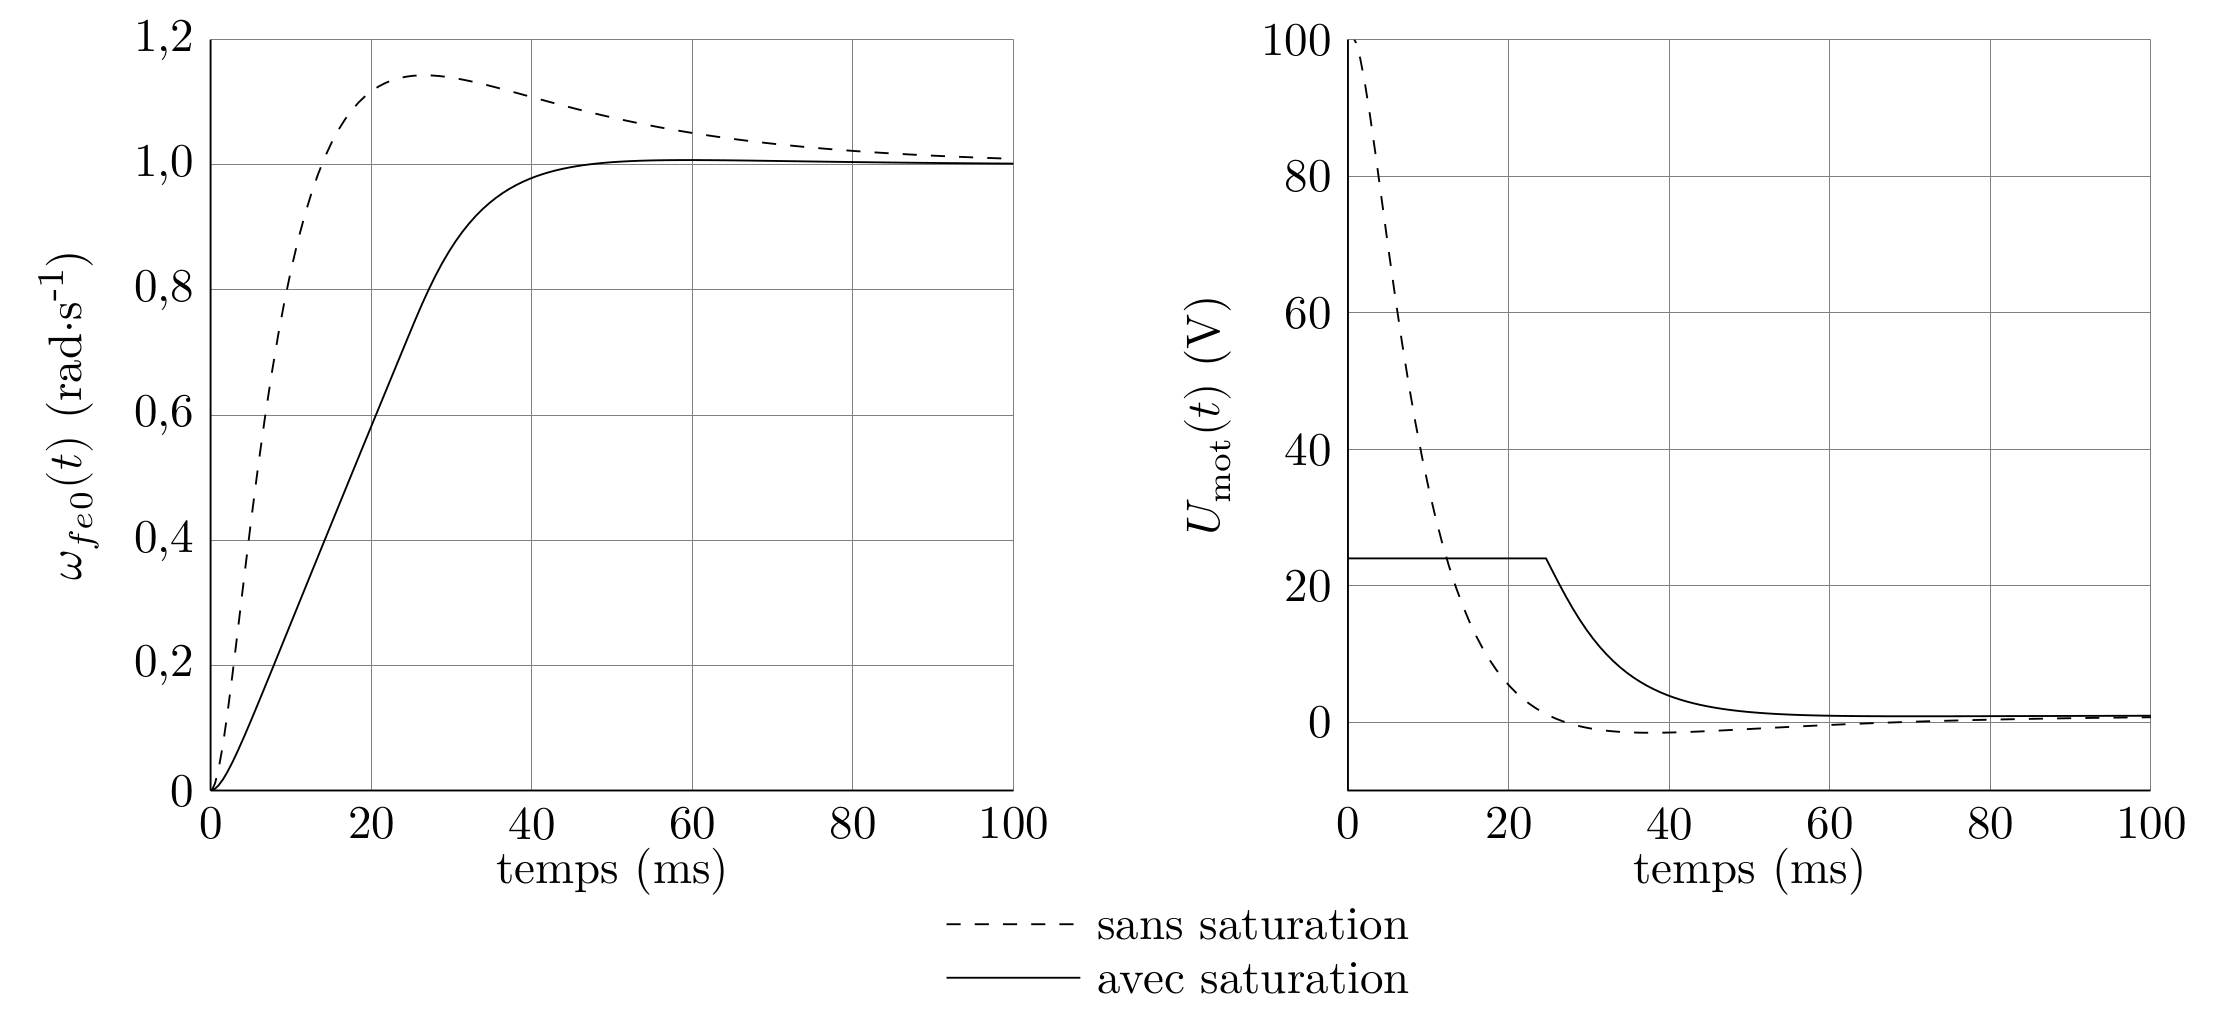
\includegraphics[width=0.7\linewidth]{img/fig15}
\captionof{figure}{\label{fig16}$\omega_{fe0}(t)$ et $U_{mot}(t)$ en fonction du temps avec et sans saturation de l'alimentation du moteur}
\end{center}

\question{Déterminer la valeur de la saturation en tension du moteur.}

\question{Donner le temps de réponse à 5\% du système avec et sans la saturation.}

\question{Que pensez-vous de l'effet de la saturation sur la précision de la réponse.}


%
%\subsection{Synthèse : validation des performances simulées du FLIR}
%
%\paragraph{Objectif:} Simuler le comportement de l'axe motorisé d'élévation du FLIR et vérifier s'il respecte le cahier des charges donné sur la figure 13.
%
%À l'instar de l'étage fin d'élévation, l'étage gros d'élévation est également asservi, mais en position angulaire. Il doit permettre à l'étage fin d'élévation de vérifier l'hypothèse émise précédemment, soit $\overrightarrow{u}\approx\overrightarrow{z_e}$, c'est-à-dire que l'angle $\beta(t)$ doit rester dans l'intervalle $[-5\textdegree, +5\textdegree]$.
%
%Un capteur LVDT (Linear Variable Differential Transformer) permet de mesurer l'écart entre l'orientation de l'étage fin d'élévation et l'étage gros d'élévation $\beta(t)=\theta_{fe0}(t)-\theta_{ge0}(t)$. Le modèle d'asservissement de l'axe motorisé d'élévation est alors celui donné sur la figure 18.
%
%\begin{center}
%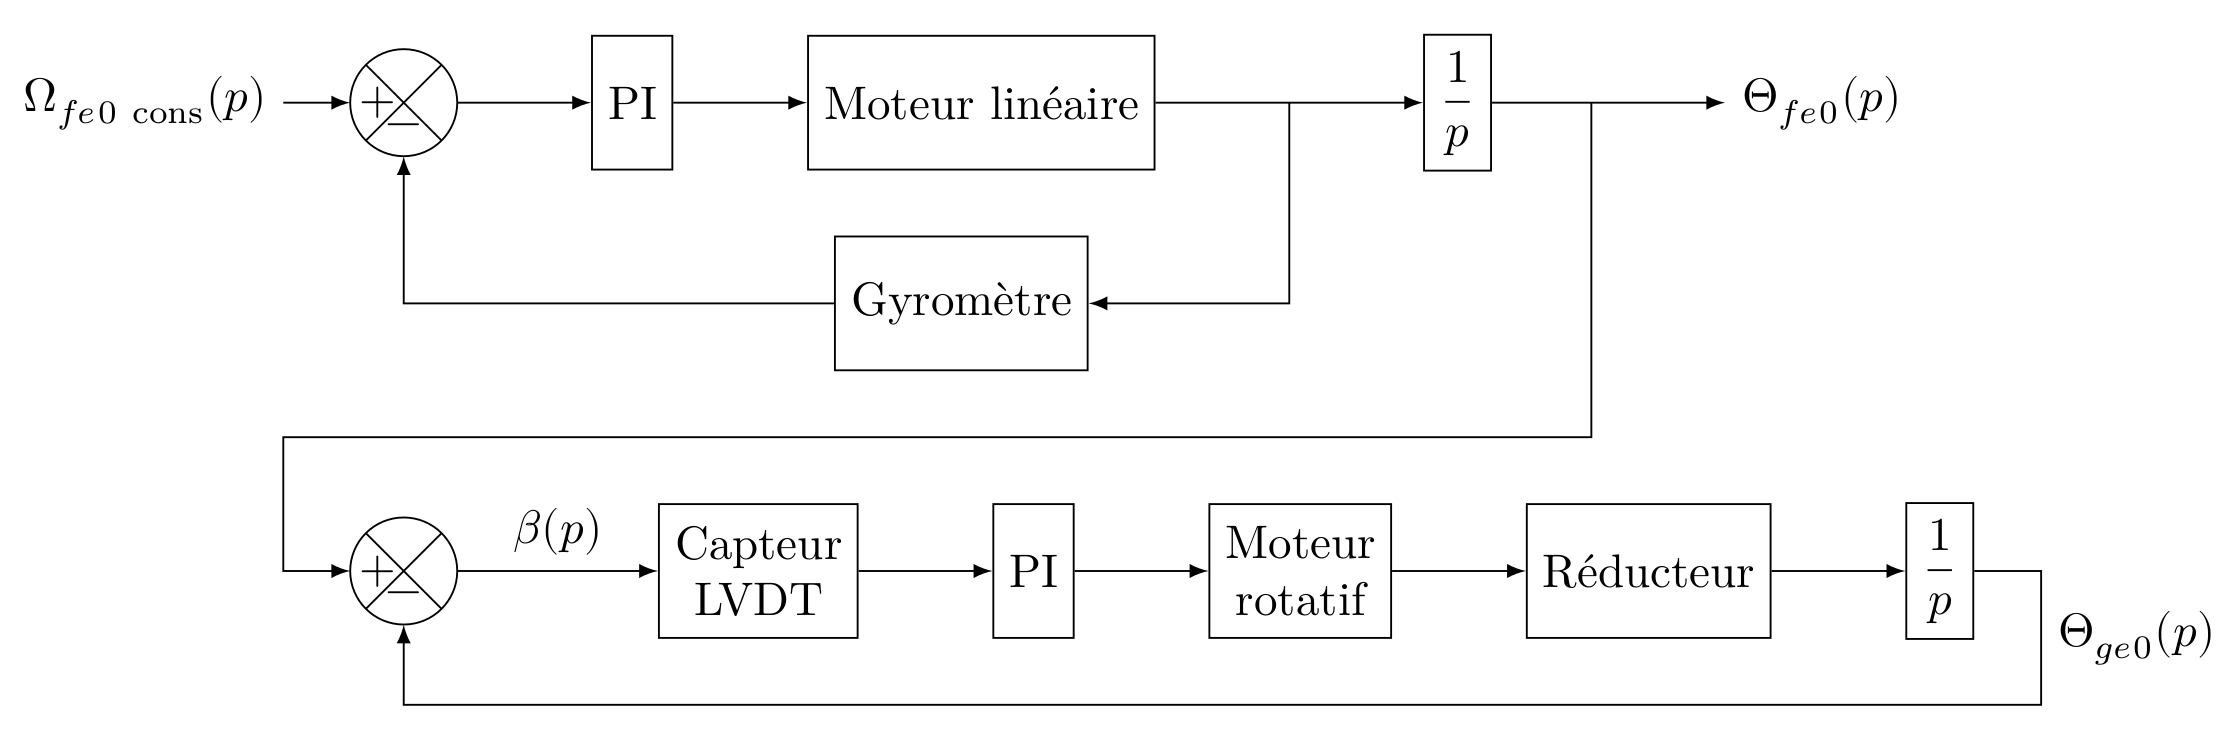
\includegraphics[width=0.7\linewidth]{img/fig16}
%\captionof{figure}{\label{fig17}Modèle d'asservissement de l'axe motorisé d'élévation, PI représente un correcteur Proportionnel Intégral}
%\end{center}
%
%La figure 19 correspond à une mesure expérimentale du taux de rotation de la tête d'un pilote pour un mouvement d'élévation de sa ligne de visée. Ce signal peut alors être utilisé comme signal de consigne envoyé à l'axe motorisé d'élévation du FLIR.
%
%\begin{center}
%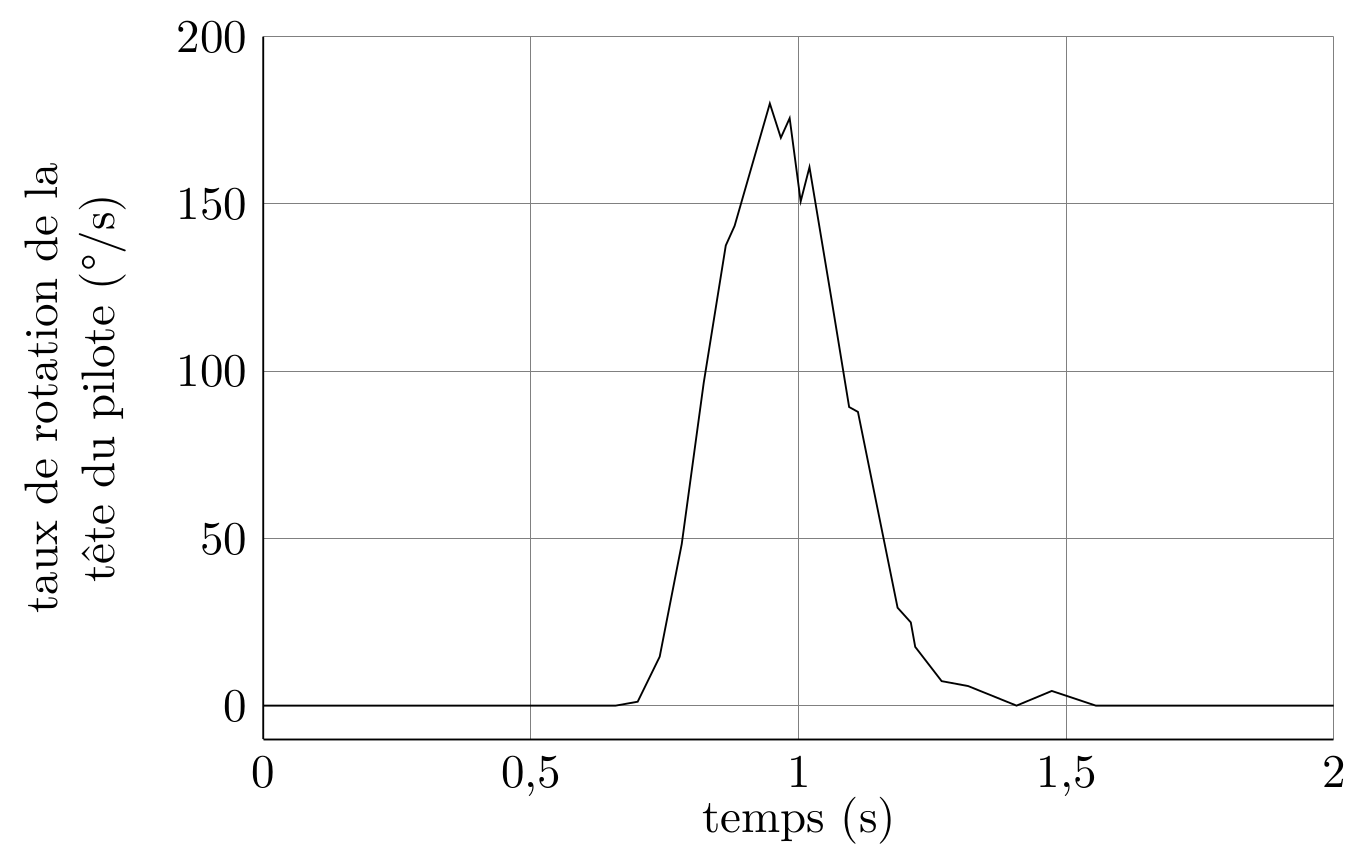
\includegraphics[width=0.7\linewidth]{img/fig17}
%\captionof{figure}{\label{fig18}Mesure expérimentale du taux de rotation de la tête du pilote (en degré par seconde) par rapport au référentiel galiléen, en fonction du temps en seconde}
%\end{center}
%
%Pour simuler le modèle de l'axe motorisé d'élévation et comparer ses performances au cahier des charges de la figure 13, il est nécessaire de définir un signal de consigne $\omega_{fe0\ cons}(t)$ composé des signaux canoniques utilisés en automatique.
%
%\question{À partir de la figure 19 et en utilisant les signaux échelon et/ou rampe, proposer un modèle temporel associé au signal de consigne $\omega_{fe0\ cons}(t)$ exprimé en $rad.s^{-1}$, sous la forme d'un tracé simple en fonction du temps en seconde. Tracer l'allure de $\theta_{fe0\ cons}(t)$, exprimé en $rad$, qui correspond à l'évolution temporelle de la ligne de visée du pilote dans ce cas. Préciser les valeurs des points caractéristiques de ces deux courbes.}
%
%\question{À partir des deux tracés précédents, indiquer quels critères du cahier des charges de la figure 13 peuvent être validés en utilisant ce signal de consigne dans la simulation du comportement de l'axe motorisé d'élévation du FLIR.}
%
%Après avoir dimensionné et implanté le correcteur proportionnel intégral (noté PI) au sein du modèle de l'étage gros d'élévation (figure 18), on simule l'évolution de $\beta(t)=\theta_{fe0}(t)-\theta_{ge0}(t)$ pour le signal de consigne $\omega_{fe0\ cons}(t)$ établi à partir de la mesure de la figure 19. Les résultats de simulation sont donnés sur la figure B du document réponse.
%
%
%\question{À partir de la figure B :
%\begin{itemize}
% \item vérifier si l'hypothèse $\overrightarrow{u}\approx \overrightarrow{z_e}$ reste valide,
% \item pour chaque critère du cahier des charges de la figure 13 et à l'aide de tracés sur le document réponse, conclure sur l'aptitude du FLIR à respecter les performances du cahier des charges en comparant les valeurs numériques mesurées sur les résultats de simulation à celles du tableau de la figure 13.
%\end{itemize}}

\section{Conception}

\question{Concevoir la fixation par vis de la caméra dont le dessin d'ensemble est présenté dans le document suivant. Il faudra compléter les vues manquantes qui ont été reportées sur le document réponse.}

\begin{center}
\huge{-- FIN --}
\end{center}

\newpage

\cleardoublepage

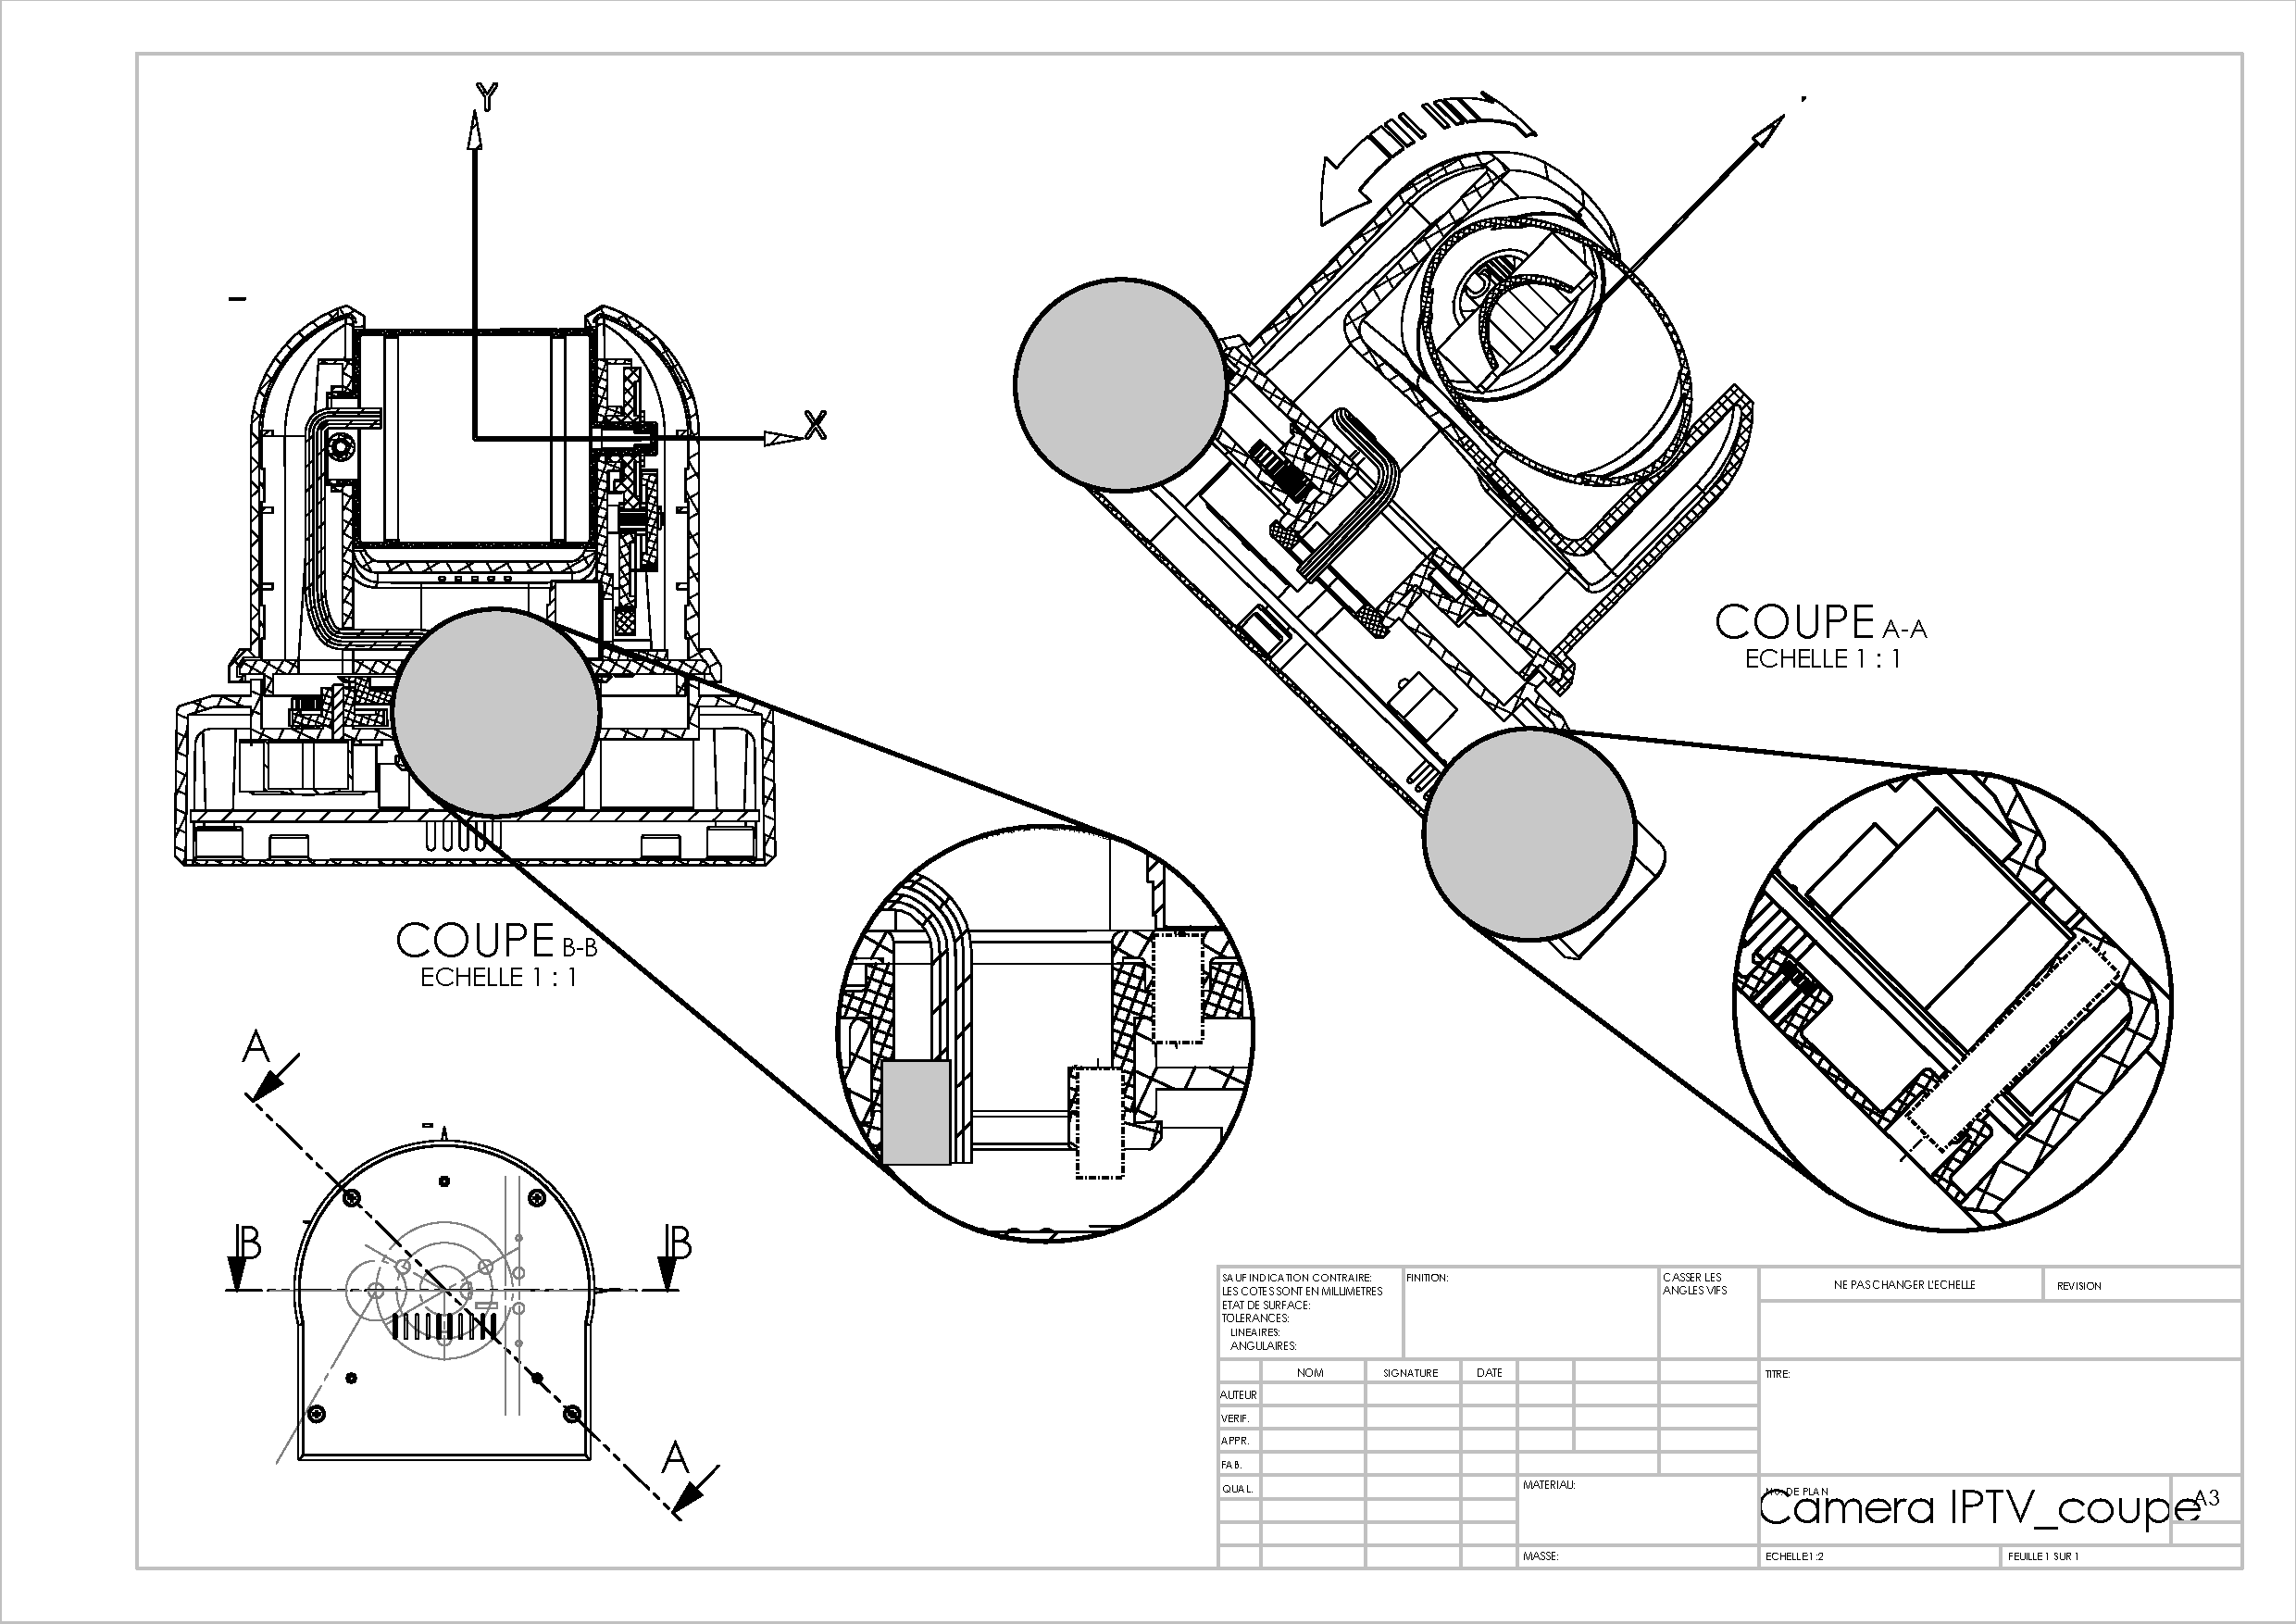
\includepdf[angle=90,offset=5mm -10mm 0mm 0mm,pages=1]{img/Dessin_DR.pdf}

\newpage
\cleardoublepage

\pagestyle{documentreponse}

\section{Document réponse}

\reponse{3}{}{Le temps maximal disponible pour l'orientation des caméras d'après la description fournie est $t_{disponible}=t_{trait}+t_{com}+t_{ddp}+t_{filtre}$ soit $t_{disponible}=80ms<120ms$.}

\reponse{5}{}{L'image a pour dimension 1024*768 pixels. Le secteur angulaire correspondant au champ de vision le plus large possible permettant la reconnaissance des mots est de 40°, ce qui conduit, à une distance de 50 mm des yeux du pilote, à une image de $\frac{50.40.\pi}{180}mm$. Donc pour un pixel la largeur est de $\frac{50.40.\pi}{180.1024}\approx0,034mm$. La résolution souhaitée étant de 1m pour un objet situé à 1km on peut en déduire qu'il faut distinguer à 50mm des yeux du pilote une taille de $\frac{50}{10^6}=0,05mm$. La taille d'un pixel étant inférieure à cette valeur, l'objet sera décrit par au moins un pixel.}


\reponse{3}{}{Il y a 1024 pixels pour un angle de 40°, soit pour 1 pixel un angle de $\frac{40.\pi}{180.1024}=7.10^{-4}rad$.}

\reponse{3}{}{Il y a en série 2 liaisons pivot d'axe orthogonaux et concourants en P. Le torseur cinématique équivalent résulte de la somme des torseurs cinématiques exprimés au point P soit $\left\{V_{leq}\right\}=\left\{\begin{array}{c}
\overrightarrow{\Omega_{charge/porteur}}=\dot\theta_{ap}.\overrightarrow{z_a}+\dot\theta_{ea}.\overrightarrow{y_a}\\
\overrightarrow{V_{P\in charge/porteur}}=\overrightarrow{O}
\end{array}
\right\}$. C'est le torseur d'une liaison sphérique à doigt de centre P d'axe et de normale .}

\newpage

\reponse{5}{}{La tête du pilote dispose d'une mobilité supplémentaire il est donc nécessaire que l'algorithme du calculateur intègre les informations de position de la tête du pilote par rapport au porteur (en particulier la position angulaire suivant la mobilité supplémentaire) fournies par le sous système de détection des postures implanté dans le casque afin de reproduire cela au niveau de l'affichage de l'image.}

\reponse{5}{
$\begin{array}{l}
A=cos\theta.cos\psi\\
B=\\
C=\\
D=\\
E=\\
F=\\
G=\\
H=\\
I=\\
\end{array}$
}{
$\begin{array}{l}
\overrightarrow{X_0}=cos\theta.cos\psi.\overrightarrow{x_p}+cos\theta.sin\psi.\overrightarrow{y_p}
-sin\theta.\overrightarrow{z_p} \\
\overrightarrow{Y_0}=[-cos\phi.sin\psi+sin\phi.sin\theta.cos\psi].\overrightarrow{x_p}
+[cos\phi.cos\psi+sin\phi.sin\theta.sin\psi].\overrightarrow{y_p}
+sin\phi.cos\theta.\overrightarrow{z_p} \\
\overrightarrow{Z_0}=[-sin\phi.sin\psi+cos\phi.sin\theta.cos\psi].\overrightarrow{x_p}
+[-sin\phi.cos\psi+cos\phi.sin\theta.sin\psi].\overrightarrow{y_p}
+cos\phi.cos\theta.\overrightarrow{z_p}
\end{array}$

On donne:\\
$\begin{array}{l}
A=cos\theta.cos\psi\\
B=cos\theta.sin\psi\\
C=-sin\theta\\
D=-cos\phi.sin\psi+sin\phi.sin\theta.cos\psi\\
E=cos\phi.cos\psi+sin\phi.sin\theta.sin\psi\\
F=sin\phi.cos\theta\\
G=sin\phi.sin\psi+cos\phi.sin\theta.cos\psi\\
H=-sin\phi.cos\psi+cos\phi.sin\theta.sin\psi\\
I=cos\phi.cos\theta \\
\end{array}$}

\reponse{4}{}{Il y a 2 liaisons sphériques en parallèle, la liaison équivalente est une liaison pivot d'axe hyperstatique de degré 1. Avantage : cela confère au système une rigidité plus importante qu'une solution isostatique et cela permet une réalisation identique pour chaque liaison élémentaire. Inconvénient : il faut gérer la contrainte géométrique de positionnement axial. La rigidité du montage permet d'être moins sensible aux perturbations extérieures et donc de conserver une précision d'orientation souhaitée malgré ces perturbations.}

\reponse{6}{}{Le champ de vecteur vitesse du mouvement de l'ensemble fin élévation donne la relation : $\overrightarrow{V_{G_{fe}\in fe/R_0}}=\overrightarrow{V_{P fe/R_0}}+\overrightarrow{\Omega_{fe/R_0}}\wedge \overrightarrow{PG_{fe}}$. Une relation de composition de mouvement conduit à : $\overrightarrow{V_{P\in porteur/R_0}}=\overrightarrow{V_{P\in porteur/axe}}+
\overrightarrow{V_{P\in axe/ge}}+\overrightarrow{V_{P\in ge/fe}}+\overrightarrow{V_{P\in fe/R_0}}
=\overrightarrow{V_{P\in fe/R_0}}=v(t).\overrightarrow{Z_0}$ (le point P ayant la particularité de se trouver à l'intersection des axes des deux rotations considérées).

Ainsi la relation permet d'écrire : soit dans la base souhaitée :\\	
$\overrightarrow{V_{G_{fe}\in fe/R_0}}=v(t).\overrightarrow{Z_0}+\dot\theta_{ea}(t).\overrightarrow{y_a}\wedge\frac{m_o.d}{m_o+m_{cyl}}.\overrightarrow{x_e}=v(t).\overrightarrow{Z_0}-\dot\theta_{ea}(t).\frac{m_o.d}{m_o+m_{cyl}}.\overrightarrow{z_e}$\\
$\overrightarrow{V_{G_{fe}\in fe/R_0}}=v(t).\overrightarrow{Z_0}-\dot\theta_{ea}(t).\frac{m_o.d}{m_o+m_{cyl}}.(sin\theta_{eo}(t).\overrightarrow{X_0}+cos\theta_{eo}(t).\overrightarrow{Z_0})$
}

\reponse{6}{}{Ayant au préalable calculé le vecteur vitesse du centre d'inertie, on peut par dérivation obtenir le vecteur accélération : 

$\overrightarrow{\Gamma_{G_{fe}\in fe/R_0}}=\gamma(t).\overrightarrow{Z_0}-\ddot\theta_{ea}(t).\frac{m_o.d}{m_o+m_{cyl}}.\overrightarrow{z_e}-\dot\theta_{ea}^2(t).\frac{m_o.d}{m_o+m_{cyl}}.\overrightarrow{x_e}$


$\overrightarrow{\Gamma_{G_{fe}\in fe/R_0}}=\gamma(t).\overrightarrow{Z_0}-\ddot\theta_{ea}(t).\frac{m_o.d}{m_o+m_{cyl}}.(sin\theta_{eo}(t).\overrightarrow{X_0}+cos\theta_{eo}(t).\overrightarrow{Z_0})-\dot\theta_{ea}^2(t).\frac{m_o.d}{m_o+m_{cyl}}.(cos\theta_{eo}(t).\overrightarrow{X_0}-sin\theta_{eo}(t).\overrightarrow{Z_0})$


$\overrightarrow{\Gamma_{G_{fe}\in fe/R_0}}=-\frac{m_o.d}{m_o+m_{cyl}}.\left(\ddot\theta_{ea}(t).sin\theta_{eo}(t)+\dot\theta_{ea}^2(t).cos\theta_{eo}(t)\right).\overrightarrow{X_0}+$\\
$\left(\gamma(t)+\frac{m_o.d}{m_o+m_{cyl}}.(-\ddot\theta_{ea}(t).cos\theta_{eo}(t)+\dot\theta_{ea}^2(t).sin\theta_{eo}(t))\right).\overrightarrow{Z_0}$
}

\reponse{4}{}{On a $\overrightarrow{V_{A\in fe/R_0}}=\overrightarrow{V_{G_{fe}\in fe/R_0}}+\overrightarrow{\Omega_{fe/R_0}}\wedge \overrightarrow{G_{fe}A}=v(t).\overrightarrow{Z_0}+r\dot\theta_{feo}.\overrightarrow{z_e}$, avec $\overrightarrow{AP}=\overrightarrow{AG_{fe}}=r.\overrightarrow{x_e}$.

Or, par composition de mouvement $\overrightarrow{V_{A,fe/R_0}}=\overrightarrow{V_{A,fe/ge}}+\overrightarrow{V_{A,ge/R_0}}=v_{tige}(t).\overrightarrow{z_e}+v(t).\overrightarrow{Z_0}$ ce qui conduit à la relation $v_{tige}(t)=r.\dot\theta_{feo}$.}

\newpage

\reponse{3}{}{On a $B_{fe}.\ddot\theta_{feo}(t)=r.F_{mot}$, donc $B_{fe}.p^2.\theta_{feo}(p)=r.F_{mot}(p)$, ce qui mène à $\frac{\Omega_{fe}(p)}{F_{mot}(p)}=\frac{r}{B_{fe}.p}$.

D'après le schéma bloc, on a $\frac{\Omega_{fe}(p)}{F_{mot}(p)}=\frac{K_1}{M_{eq}.p}$, ainsi, $K_1=\frac{1}{r}(m^{-1})$ et $M_{eq}=\frac{B_{fe}}{r^2}(kg)$.
}


\reponse{2}{}{Le gyromètre est modélisé par une fonction de transfert du 1er ordre, la pulsation de coupure à -3dB est directement donnée par $\frac{1}{\tau_{gyro}}$ d'où $\tau_{gyro}=\frac{1}{2.\pi.f}=\frac{1}{2.\pi.100}\approx 1,6(ms)$.}

\reponse{4}{}{$FTBF(p)=\frac{\frac{\frac{K_{fe}}{R_{fe}.M_{eq}.p}}{1+\frac{K_{fe}}{R_{fe}.M_{eq}.p}.K_{fe}}.K_1}{1+\frac{\frac{K_{fe}}{R_{fe}.M_{eq}.p}}{1+\frac{K_{fe}}{R_{fe}.M_{eq}.p}.K_{fe}.K_1}.\frac{1}{1+\tau_{gyro}}}=\frac{K_{fe}.K_1.(1+\tau_{gyro}.p)}{K_{fe}.K_1+K^2_{fe}+(R_{fe}.M_{eq}+\tau_{gyro}.K^2_{fe}).p+R_{fe}.M_{eq}.\tau_{gyro}.p^2}$

Soit:
$FTBF(p)=\frac{K_1}{K_1+K_{fe}}.\frac{1+\tau_{gyro}.p}{1+\frac{R_{fe}.M_{eq}+\tau_{gyro}.K^2_{fe}}{K_{fe}.K_1+K^2_{fe}}.p+\frac{R_{fe}.M_{eq}.\tau_{gyro}}{K_{fe}.K_1+K^2_{fe}}.p^2}$
}

\reponse{3}{}{D'après la fonction de transfert proposée, on peut déterminer la pulsation propre non amortie du système $\omega_n=\sqrt{\frac{1}{6.10^{-4}}}\approx40rad.s^{-1}$ et l'amortissement $m=\frac{\omega_n}{2}.3,65.10^{-1}\approx7,3$. Ce qui à l'aide de l'abaque permet de déterminer le temps de réponse réduit $t_{5\%}.\omega_n\approx 45$ d'où $t_{5\%}\approx\frac{45}{40}\approx1,1s$. Le critère du temps de réponse de <40ms n'est pas respecté. De plus l'écart statique vaut $1-0,5.1=0,5\neq0$ ce qui ne respecte pas le cahier des charges.}


%\reponse{4}{
%\begin{center}
% 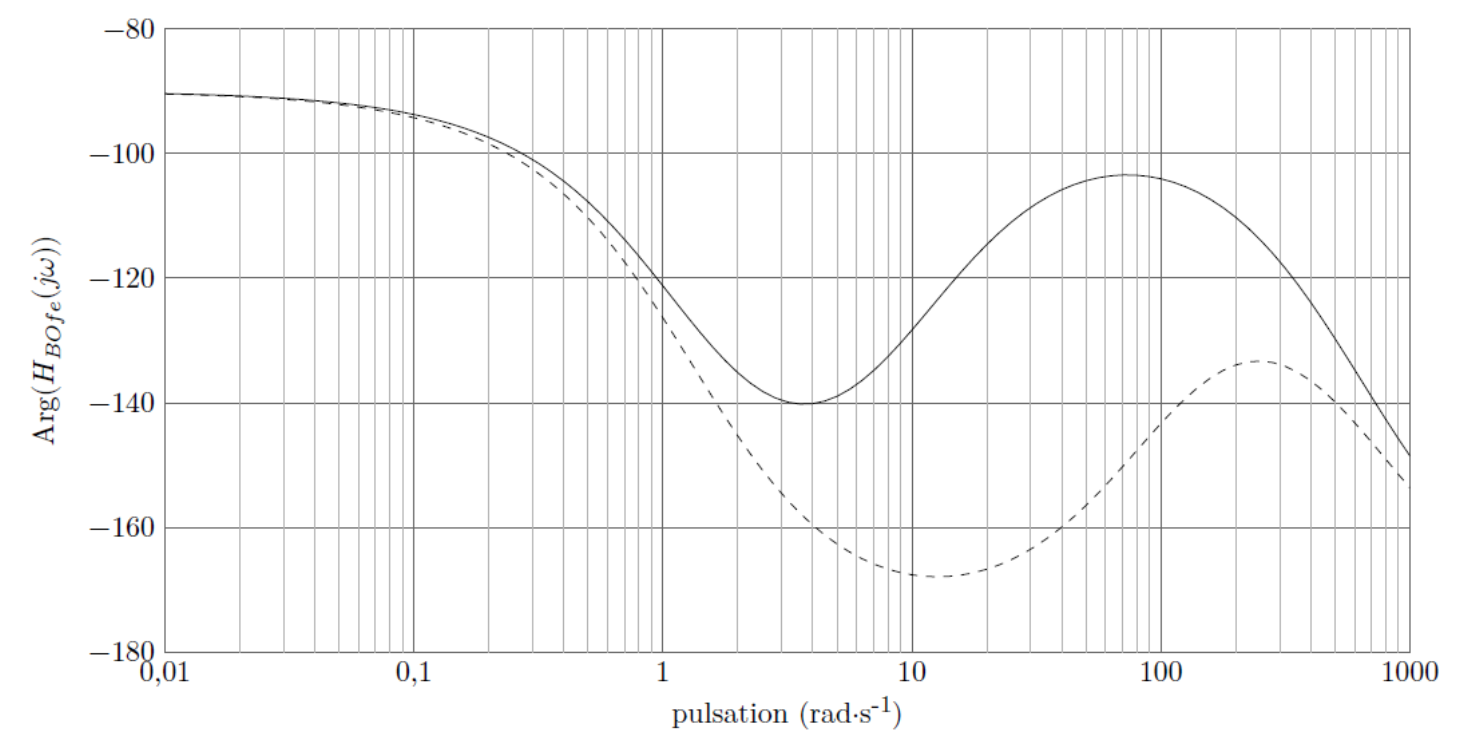
\includegraphics[width=0.8\linewidth]{img/TTQFGQ}
%\end{center}
%}{
%\begin{center}
% 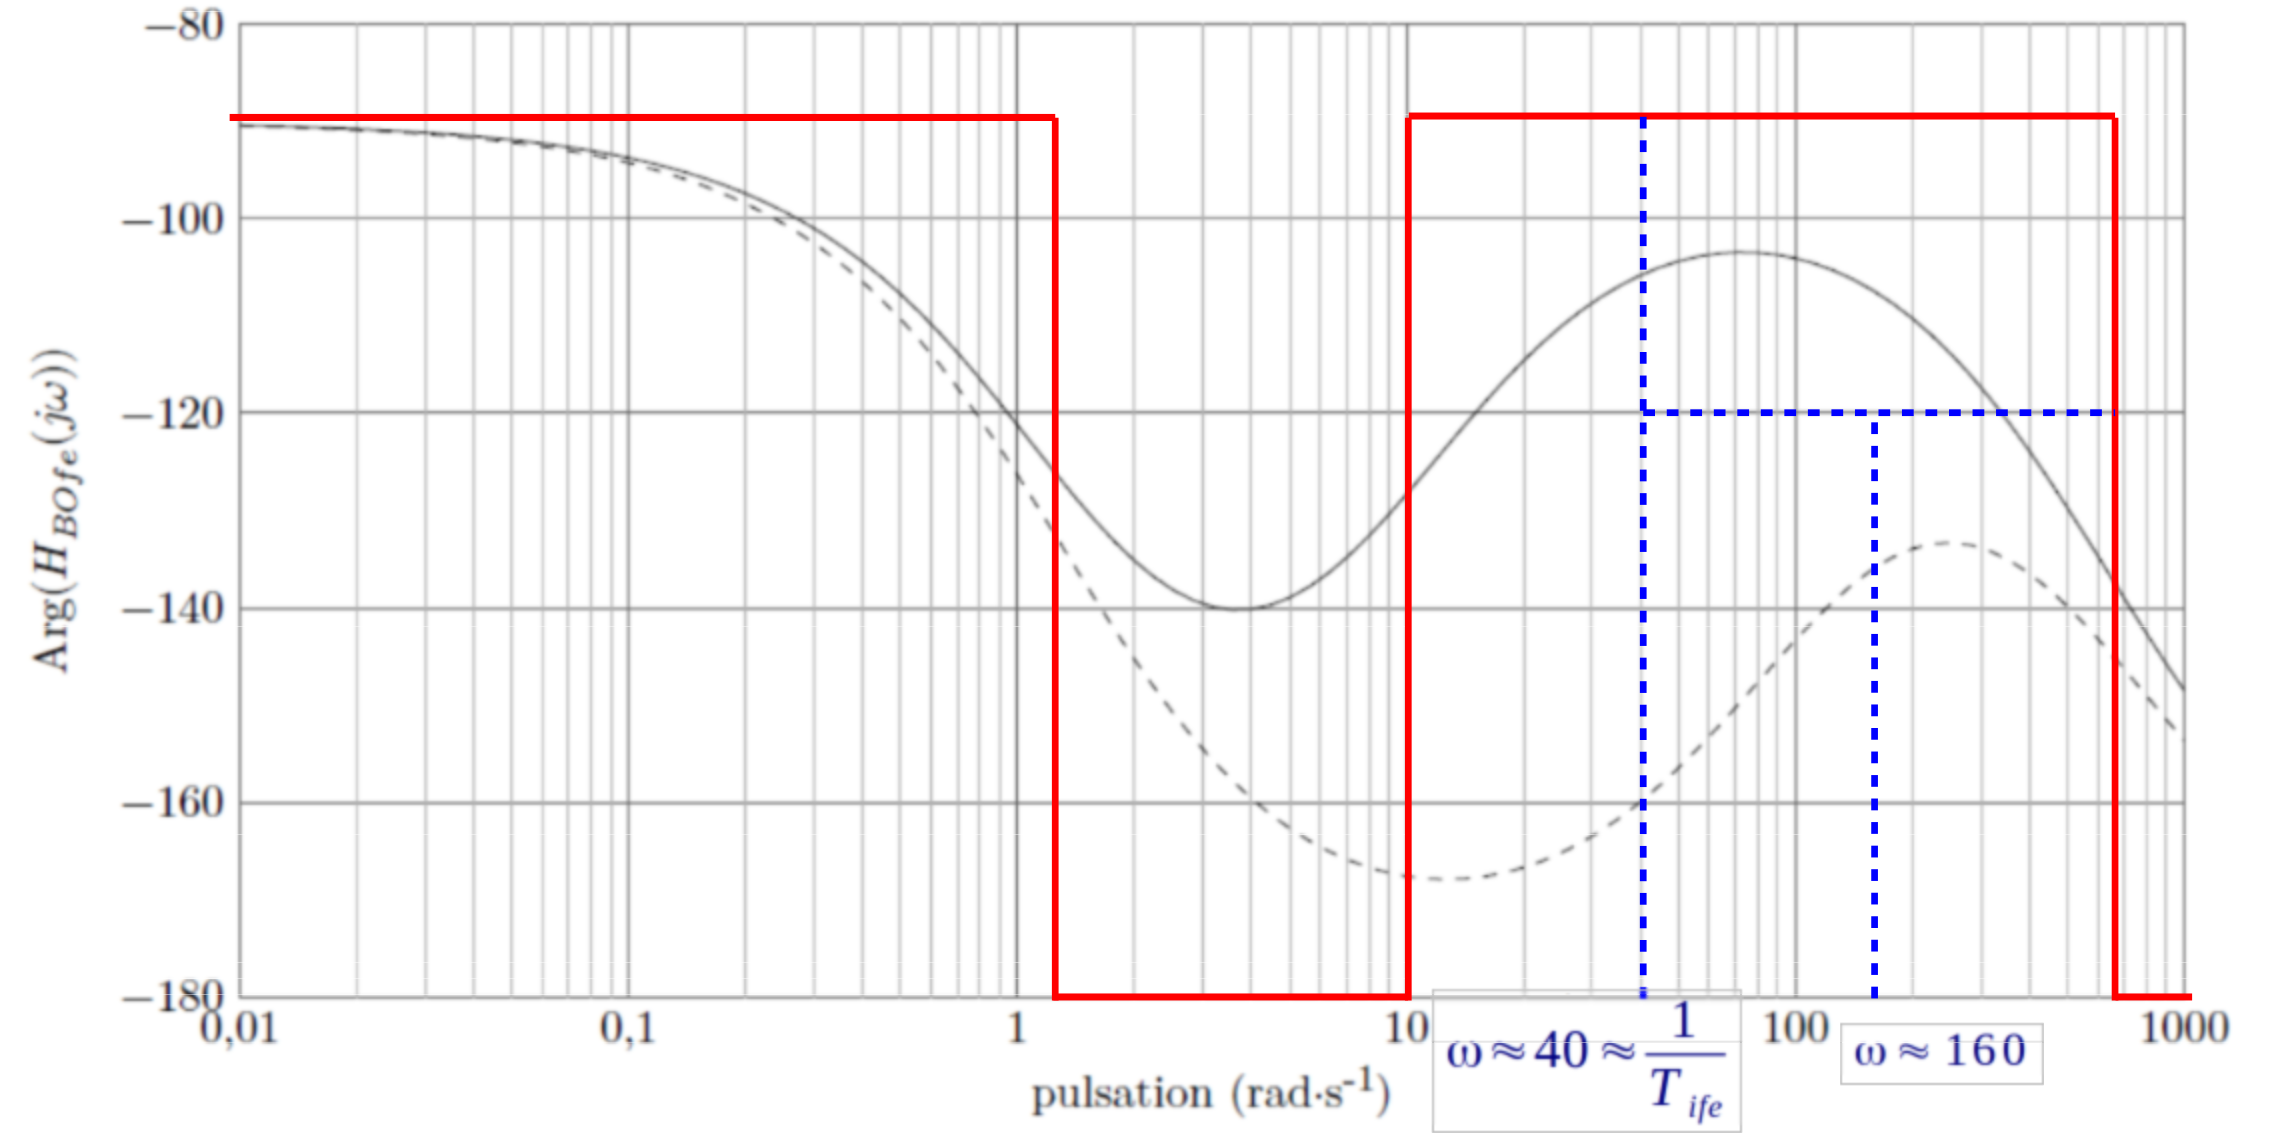
\includegraphics[width=0.8\linewidth]{img/TTQFGQ_cor}
%\end{center}
%
%La fonction de transfert comporte un terme en 1/p qui aux basses pulsations induit un déphasage de -90°, puis un 1er ordre qui à partir de $\frac{1}{0,75}=1,33rad.s^{-1}$ induit -90° de plus. Enfin le pseudo dérivateur induit +90° à partir de $\frac{1}{T_{ife}}=10rad.s^{-1}$ et le dernier terme correspondant à un 1er ordre rajoute -90° à partir de $\omega=625rad.s^{-1}$.}


\reponse{2}{}{$1+\frac{1}{T_{ife}.p}=\frac{T_{ife}.p}{T_{ife}.p}+\frac{1}{T_{ife}.p}=\frac{T_{ife}.p+1}{T_{ife}.p}$ on retrouve ainsi la forme demandée.}

\newpage

\reponse{0}{
\begin{center}
\begin{tikzpicture}[xscale=7/4]
\begin{scope}[yscale=3/120]
\OrdBode{20}
\semilog{-2}{3}{-100}{20}
\end{scope}

\begin{scope}[yshift=-3.5cm,yscale=3/90]
\semilog{-2}{3}{-90}{0}
\end{scope}
\end{tikzpicture}
\end{center}}
{
\begin{center}
\begin{tikzpicture}[xscale=7/4]
\begin{scope}[yscale=3/120]
\OrdBode{20}
\semilog{-2}{3}{-100}{20}
\BodeGraph[asymp lines,samples=100]{-2:3}{\POAmpAsymp{1}{0.75}}
\BodeGraph{-2:3}{\POAmp{1}{0.75}}
\end{scope}

\begin{scope}[yshift=-3.5cm,yscale=3/90]
\semilog{-2}{3}{-90}{0}
\BodeGraph[asymp lines,samples=100, const plot]{-2:3}{\POArgAsymp{1}{0.75}}
\BodeGraph{-2:3}{\POArg{1}{0.75}}
\end{scope}
\end{tikzpicture}
\end{center}}

\reponse{0}{
\begin{center}
\begin{tikzpicture}[xscale=7/4]
\begin{scope}[yscale=3/30]
\UnitedB
\semilog{-2}{3}{0}{30}\end{scope}
\begin{scope}[yshift=-3.5cm,yscale=3/90]
\UniteDegre\semilog{-2}{3}{0}{90}
\end{scope}
\end{tikzpicture}
\end{center}}
{
\begin{center}
\begin{tikzpicture}[xscale=7/4]
\begin{scope}[yscale=3/30]
\UnitedB
\BodeGraph[thick]{-2:3}{\PDAmp{1}{0.01}}
\BodeGraph[black]{-2:3}{\PDAmpAsymp{1}{0.01}}
\semilog{-2}{3}{0}{30}\end{scope}
\begin{scope}[yshift=-3.5cm,yscale=3/90]
\UniteDegre\semilog{-2}{3}{0}{90}
\BodeGraph[thick]{-2:3}{\PDArg{1}{0.01}}
\BodeGraph[samples=2,black,samples=201]{-2:3}{\PDArgAsymp{1}{0.01}}
\end{scope}
\end{tikzpicture}
\end{center}}

\newpage

\reponse{0}{
\begin{center}
\begin{tikzpicture}[xscale=7/4]
\begin{scope}[yscale=3/70]
\UnitedB
\semilog{-2}{3}{-50}{20}\end{scope}
\begin{scope}[yshift=-3.5cm,yscale=3/90]
\UniteDegre\semilog{-2}{3}{-90}{0}
\end{scope}
\end{tikzpicture}
\end{center}}
{
\begin{center}
\begin{tikzpicture}[xscale=7/4]
\begin{scope}[yscale=3/70]
\UnitedB
\BodeGraph[thick]{-2:3}{\PDAmp{1}{0.01}+\POAmp{1}{0.75}}
\BodeGraph[black]{-2:3}{\PDAmpAsymp{1}{0.01}+\POAmpAsymp{1}{0.75}}
\semilog{-2}{3}{-50}{20}\end{scope}
\begin{scope}[yshift=-3.5cm,yscale=3/90]
\UniteDegre\semilog{-2}{3}{-90}{0}
\BodeGraph[thick]{-2:3}{\PDArg{1}{0.01}\POArg{1}{0.75}}
\BodeGraph[samples=2,black,samples=201]{-2:3}{\PDArgAsymp{1}{0.01}+\POArgAsymp{1}{0.75}}
\end{scope}
\end{tikzpicture}
\end{center}}

\reponse{0}{
\begin{center}
\begin{tikzpicture}[xscale=12/4]
\begin{scope}[yscale=6/240]
\OrdBode{50}
\semilog{-2}{3}{-150}{100}
\BodeGraph{-2:3}{\IntAmp{1}+\POAmp{10}{0.0016}+\POAmp{1}{0.75}+\PDAmp{1}{0.1}}
\end{scope}

\begin{scope}[yshift=-2.5cm,yscale=3/100]
\OrdBode{20}
\semilog{-2}{3}{-180}{-80}
\BodeGraph{-2:3}{\IntArg{10}+\POArg{1}{0.0016}+\POArg{1}{0.75}+\PDArg{1}{0.1}}
\end{scope}
\end{tikzpicture}
\end{center}}
{\begin{center}
\begin{tikzpicture}[xscale=12/4]
\begin{scope}[yscale=6/240]
\OrdBode{50}
\semilog{-2}{3}{-150}{100}
\BodeGraph[asymp lines,samples=100]{-2:3}{\IntAmp{10}+\POAmpAsymp{1}{0.0016}+\POAmpAsymp{1}{0.75}+\PDAmpAsymp{1}{0.1}}
\BodeGraph{-2:3}{\IntAmp{1}+\POAmp{10}{0.0016}+\POAmp{1}{0.75}+\PDAmp{1}{0.1}}
\end{scope}

\begin{scope}[yshift=-2.5cm,yscale=3/100]
\OrdBode{20}
\semilog{-2}{3}{-180}{-80}
\BodeGraph[asymp lines,samples=100, const plot]{-2:3}{\IntArg{10}+\POArgAsymp{1}{0.0016}+\POArgAsymp{1}{0.75}+\PDArgAsymp{1}{0.1}}
\BodeGraph{-2:3}{\IntArg{10}+\POArg{1}{0.0016}+\POArg{1}{0.75}+\PDArg{1}{0.1}}
\end{scope}
\end{tikzpicture}
\end{center}}

\reponse{4}{}{Par identification, on voit que la courbe de la phase passe de -180° à -90° pour $\omega=10^1rad.s^{-1}$, on en déduit donc que $T_{ife}=0,1s$.

On constate de plus que sur le tracé asymptotique, pour $\omega=1rad.s^{-1}$, on peut assimiler
$20.log(|H_{BOfe}(p)|)$ à $\frac{K_{pfe}}{T_{ife}.p}$, ainsi, $20.log\left(\frac{K_{pfe}}{T_{ife}}\right)\approx20$, donc, $\frac{K_{pfe}}{T_{ife}}=10$, donc $K_{pfe}=1$.
}

\reponse{2}{}{La seconde courbe montre une saturation à 24V.}

\reponse{2}{}{Sur la première courbe, on voit que le temps de réponse à 5\% est d'environ 35ms avec la saturation et 50ms sans.}

\reponse{2}{}{La saturation n'a aucun effet sur la précision de la réponse.}

\newpage

\vspace{-2cm}

\reponse{0}{
\begin{center}
 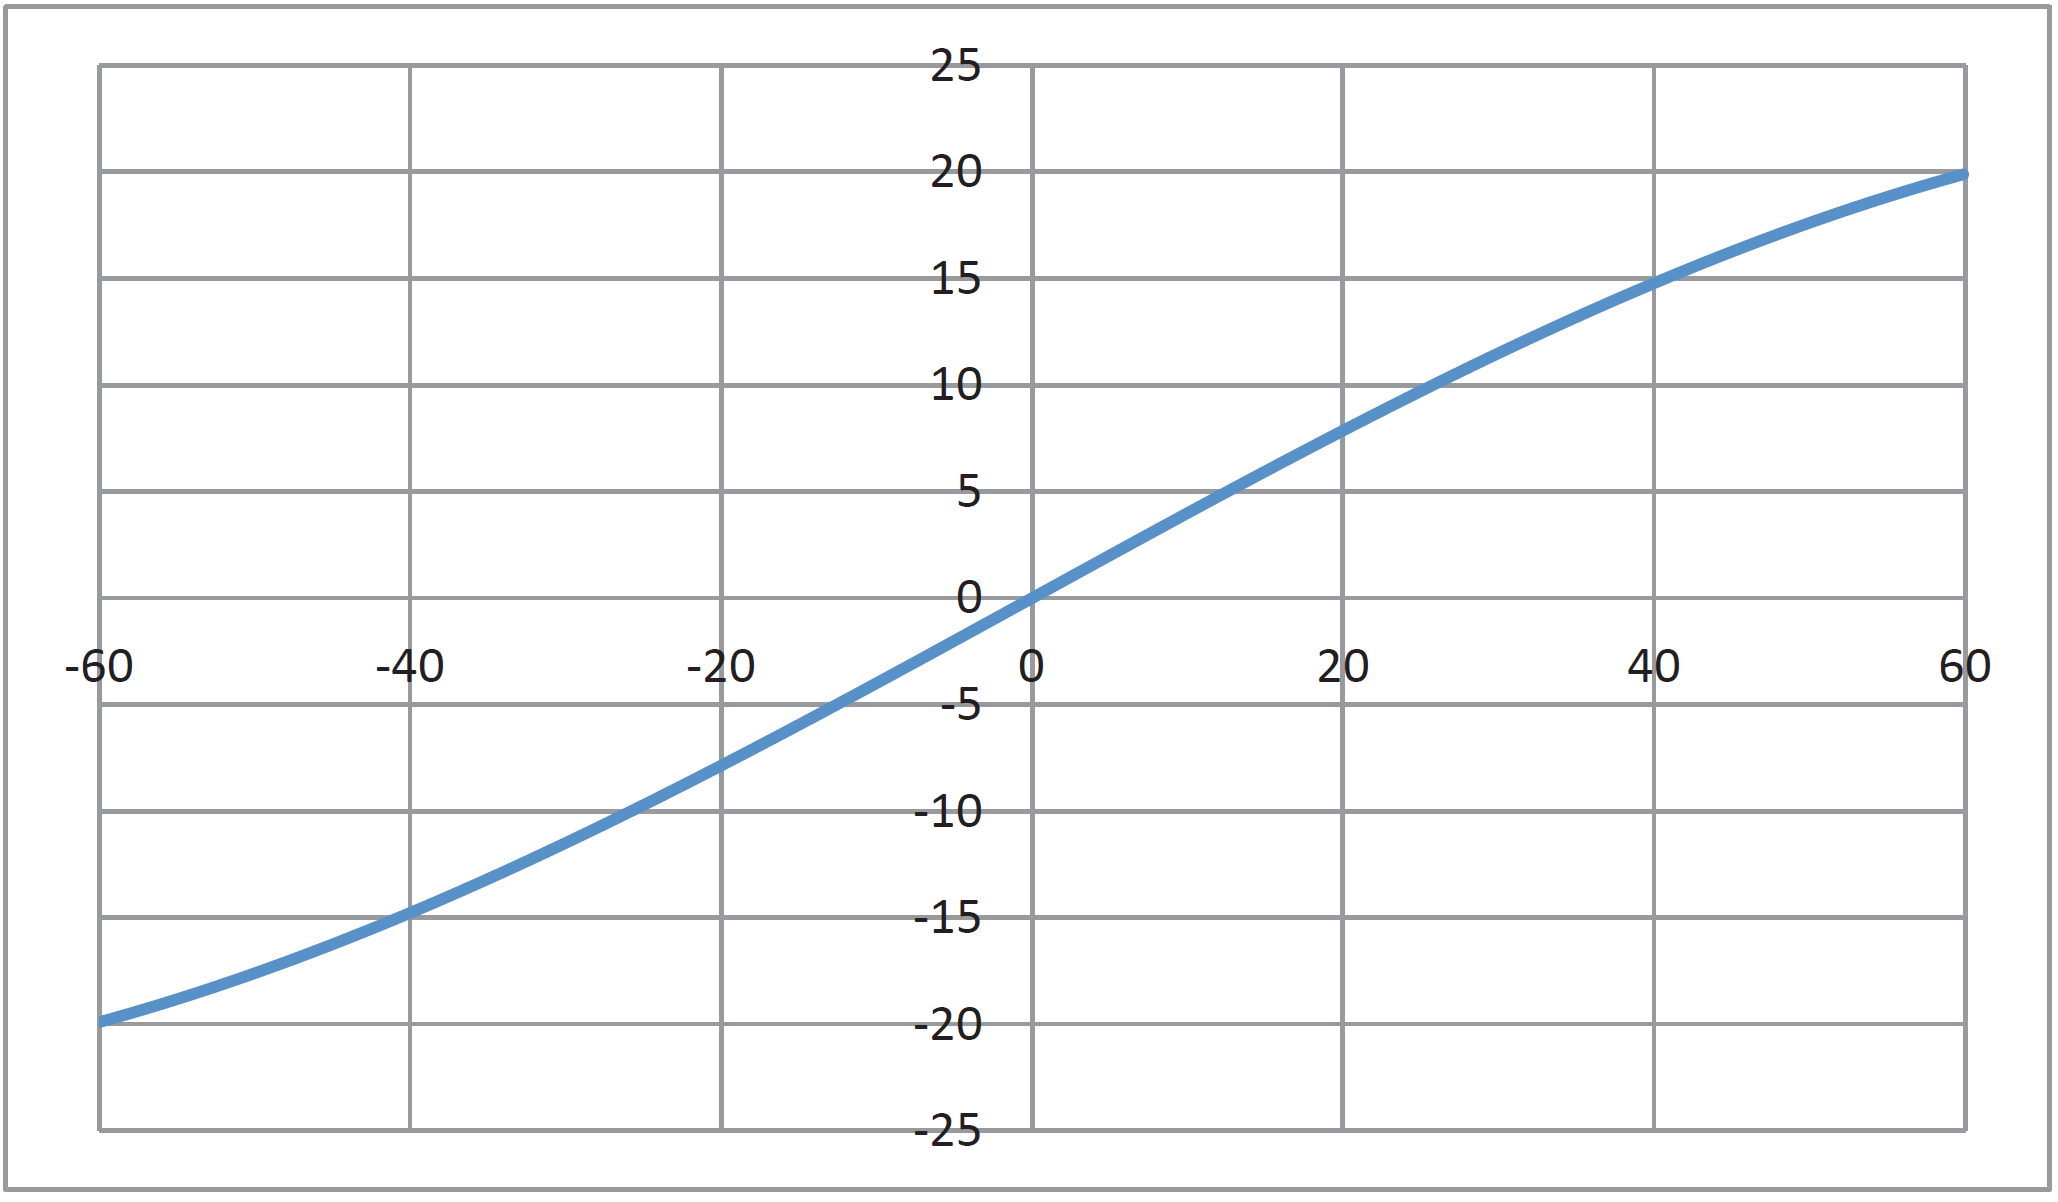
\includegraphics[width=0.6\linewidth]{img/DR1}\\
 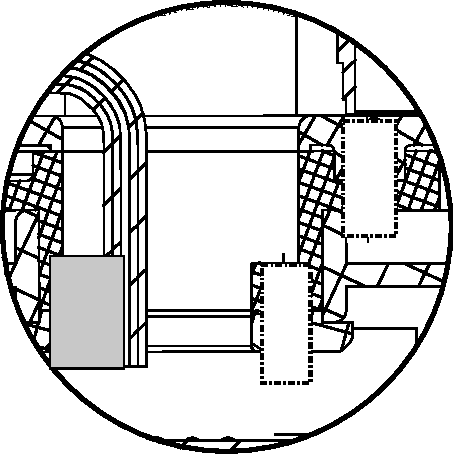
\includegraphics[width=0.6\linewidth]{img/DR2}
\end{center}
}{
\begin{center}
 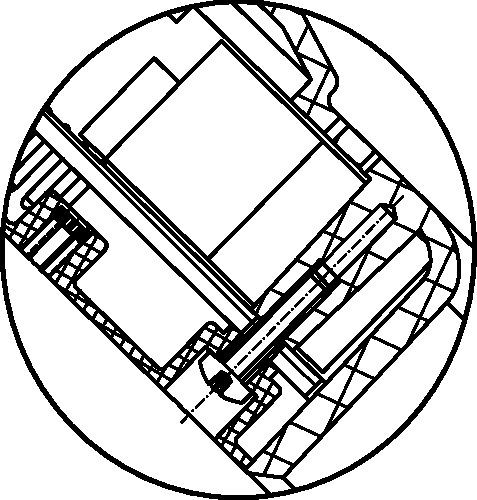
\includegraphics[width=0.6\linewidth]{img/DR1_cor}\\
 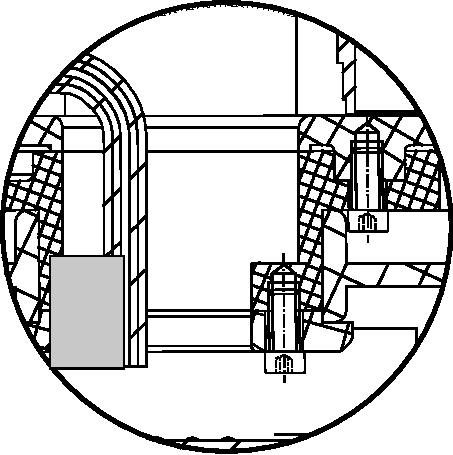
\includegraphics[width=0.6\linewidth]{img/DR2_cor}
\end{center}
}


\end{document}
